% Options for packages loaded elsewhere
\PassOptionsToPackage{unicode}{hyperref}
\PassOptionsToPackage{hyphens}{url}
%
\documentclass[
]{article}
\usepackage{amsmath,amssymb}
\usepackage{iftex}
\ifPDFTeX
  \usepackage[T1]{fontenc}
  \usepackage[utf8]{inputenc}
  \usepackage{textcomp} % provide euro and other symbols
\else % if luatex or xetex
  \usepackage{unicode-math} % this also loads fontspec
  \defaultfontfeatures{Scale=MatchLowercase}
  \defaultfontfeatures[\rmfamily]{Ligatures=TeX,Scale=1}
\fi
\usepackage{lmodern}
\ifPDFTeX\else
  % xetex/luatex font selection
\fi
% Use upquote if available, for straight quotes in verbatim environments
\IfFileExists{upquote.sty}{\usepackage{upquote}}{}
\IfFileExists{microtype.sty}{% use microtype if available
  \usepackage[]{microtype}
  \UseMicrotypeSet[protrusion]{basicmath} % disable protrusion for tt fonts
}{}
\makeatletter
\@ifundefined{KOMAClassName}{% if non-KOMA class
  \IfFileExists{parskip.sty}{%
    \usepackage{parskip}
  }{% else
    \setlength{\parindent}{0pt}
    \setlength{\parskip}{6pt plus 2pt minus 1pt}}
}{% if KOMA class
  \KOMAoptions{parskip=half}}
\makeatother
\usepackage{xcolor}
\usepackage[margin=1in]{geometry}
\usepackage{longtable,booktabs,array}
\usepackage{calc} % for calculating minipage widths
% Correct order of tables after \paragraph or \subparagraph
\usepackage{etoolbox}
\makeatletter
\patchcmd\longtable{\par}{\if@noskipsec\mbox{}\fi\par}{}{}
\makeatother
% Allow footnotes in longtable head/foot
\IfFileExists{footnotehyper.sty}{\usepackage{footnotehyper}}{\usepackage{footnote}}
\makesavenoteenv{longtable}
\usepackage{graphicx}
\makeatletter
\def\maxwidth{\ifdim\Gin@nat@width>\linewidth\linewidth\else\Gin@nat@width\fi}
\def\maxheight{\ifdim\Gin@nat@height>\textheight\textheight\else\Gin@nat@height\fi}
\makeatother
% Scale images if necessary, so that they will not overflow the page
% margins by default, and it is still possible to overwrite the defaults
% using explicit options in \includegraphics[width, height, ...]{}
\setkeys{Gin}{width=\maxwidth,height=\maxheight,keepaspectratio}
% Set default figure placement to htbp
\makeatletter
\def\fps@figure{htbp}
\makeatother
\setlength{\emergencystretch}{3em} % prevent overfull lines
\providecommand{\tightlist}{%
  \setlength{\itemsep}{0pt}\setlength{\parskip}{0pt}}
\setcounter{secnumdepth}{5}
\usepackage{booktabs}
\usepackage{longtable}
\usepackage{array}
\usepackage{multirow}
\usepackage{wrapfig}
\usepackage{float}
\usepackage{colortbl}
\usepackage{pdflscape}
\usepackage{tabu}
\usepackage{threeparttable}
\usepackage{threeparttablex}
\usepackage[normalem]{ulem}
\usepackage{makecell}
\usepackage{xcolor}
\ifLuaTeX
  \usepackage{selnolig}  % disable illegal ligatures
\fi
\usepackage{bookmark}
\IfFileExists{xurl.sty}{\usepackage{xurl}}{} % add URL line breaks if available
\urlstyle{same}
\hypersetup{
  pdftitle={Mid-Semester Course Evaluation Results},
  hidelinks,
  pdfcreator={LaTeX via pandoc}}

\title{Mid-Semester Course Evaluation Results}
\author{}
\date{\vspace{-2.5em}}

\begin{document}
\maketitle

{
\setcounter{tocdepth}{2}
\tableofcontents
}
\begin{longtable}[]{@{}
  >{\raggedright\arraybackslash}p{(\columnwidth - 2\tabcolsep) * \real{0.5488}}
  >{\raggedright\arraybackslash}p{(\columnwidth - 2\tabcolsep) * \real{0.4512}}@{}}
\toprule\noalign{}
\endhead
\bottomrule\noalign{}
\endlastfoot
\textbf{Course} & Business Intelligence II \\
\textbf{Course Code} & BBT4206 \\
\textbf{Class} & BBIT 4.2 \\
\textbf{Semester Duration} & 21\textsuperscript{st} August 2023 to
28\textsuperscript{th} November 2023 \\
\textbf{Date of Evaluation} &
\begin{minipage}[t]{\linewidth}\raggedright
25\textsuperscript{th} September 2023 to 4\textsuperscript{th} October
2023\\
(Week 6 \& 7 of 14)\strut
\end{minipage} \\
\textbf{Total number of students who submitted the course evaluation} &
102 \\
\textbf{Total number of students registered in the AMS at the time of
the course evaluation} & 115 \\
\textbf{Response rate} & 88.69\% \\
\textbf{e-Learning URL} &
\url{https://elearning.strathmore.edu/course/view.php?id=6599} \\
\begin{minipage}[t]{\linewidth}\raggedright
\textbf{Data collection tool URL\\
(for access to the raw data)}\strut
\end{minipage} &
\url{https://elearning.strathmore.edu/mod/questionnaire/view.php?id=221958} \\
\textbf{Lecturer} & Dr Allan Omondi
\textless aomondi@strathmore.edu\textgreater{} \\
\end{longtable}

\begin{center}\rule{0.5\linewidth}{0.5pt}\end{center}

\section{Course Evaluation Score}\label{course-evaluation-score}

Mean Course Evaluation Score = 4.3770 / 5

Percentage Mean Course Evaluation Score = 87.54\%

Median Course Evaluation Score = 4.3636 / 5

\begin{center}\rule{0.5\linewidth}{0.5pt}\end{center}

\newpage

\section{Quantitative Data Analysis}\label{quantitative-data-analysis}

\subsection{Course Evaluation Scores per
Group}\label{course-evaluation-scores-per-group}

The \textbf{``Average Course Evaluation Rating''} variable in the plot
below indicates the score \textbf{per group} with a baseline of 4/5.

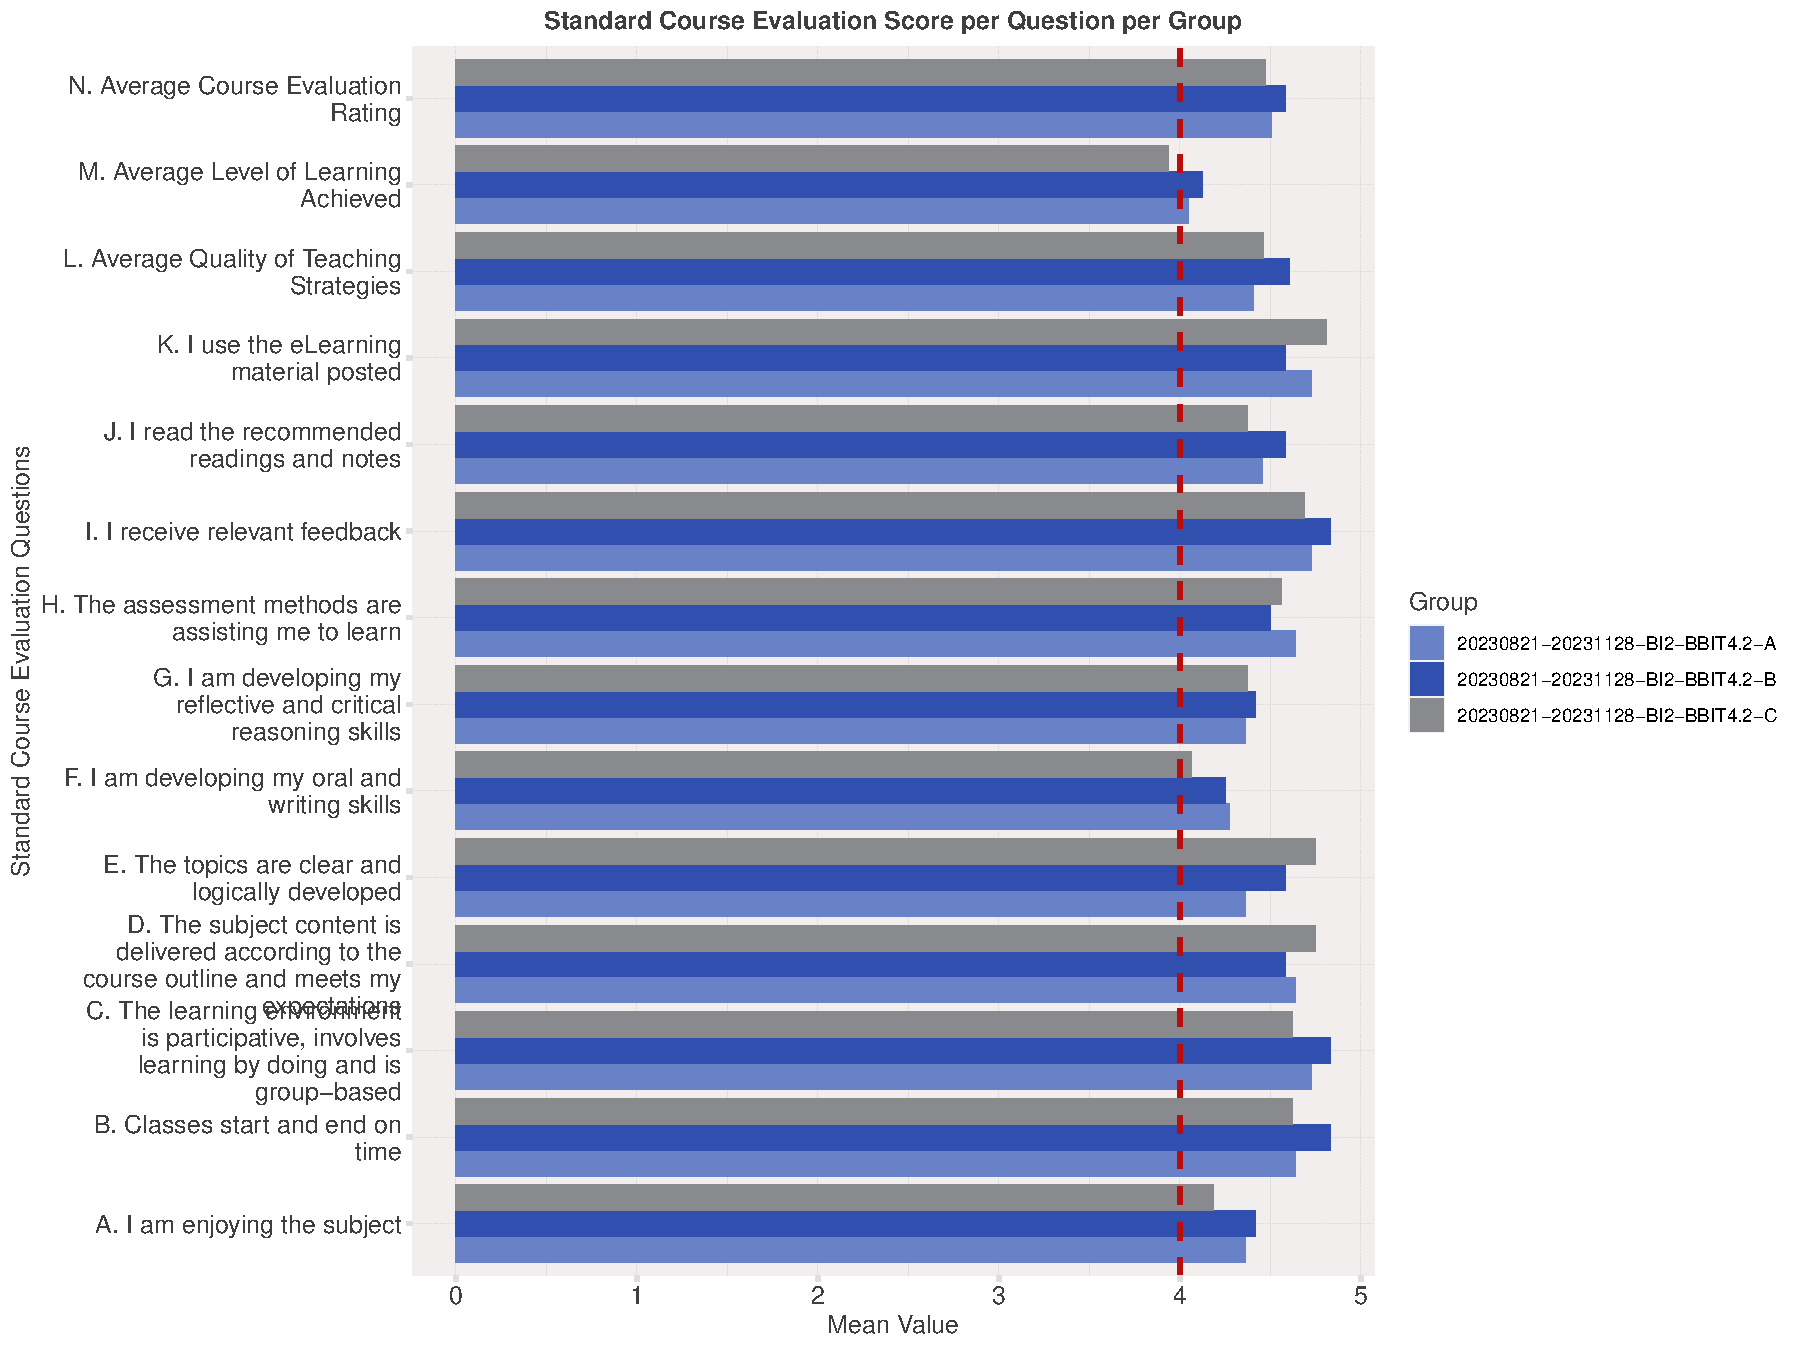
\includegraphics{AnalysisOfCourseEvaluation-Notebook_files/figure-latex/VisualizationsForCourseEvaluationResultsperClassGroup-1.pdf}

\newpage

The \textbf{``Average Course Evaluation Rating''} variable in the plot
below indicates the score \textbf{per gender} with a baseline of 4/5.

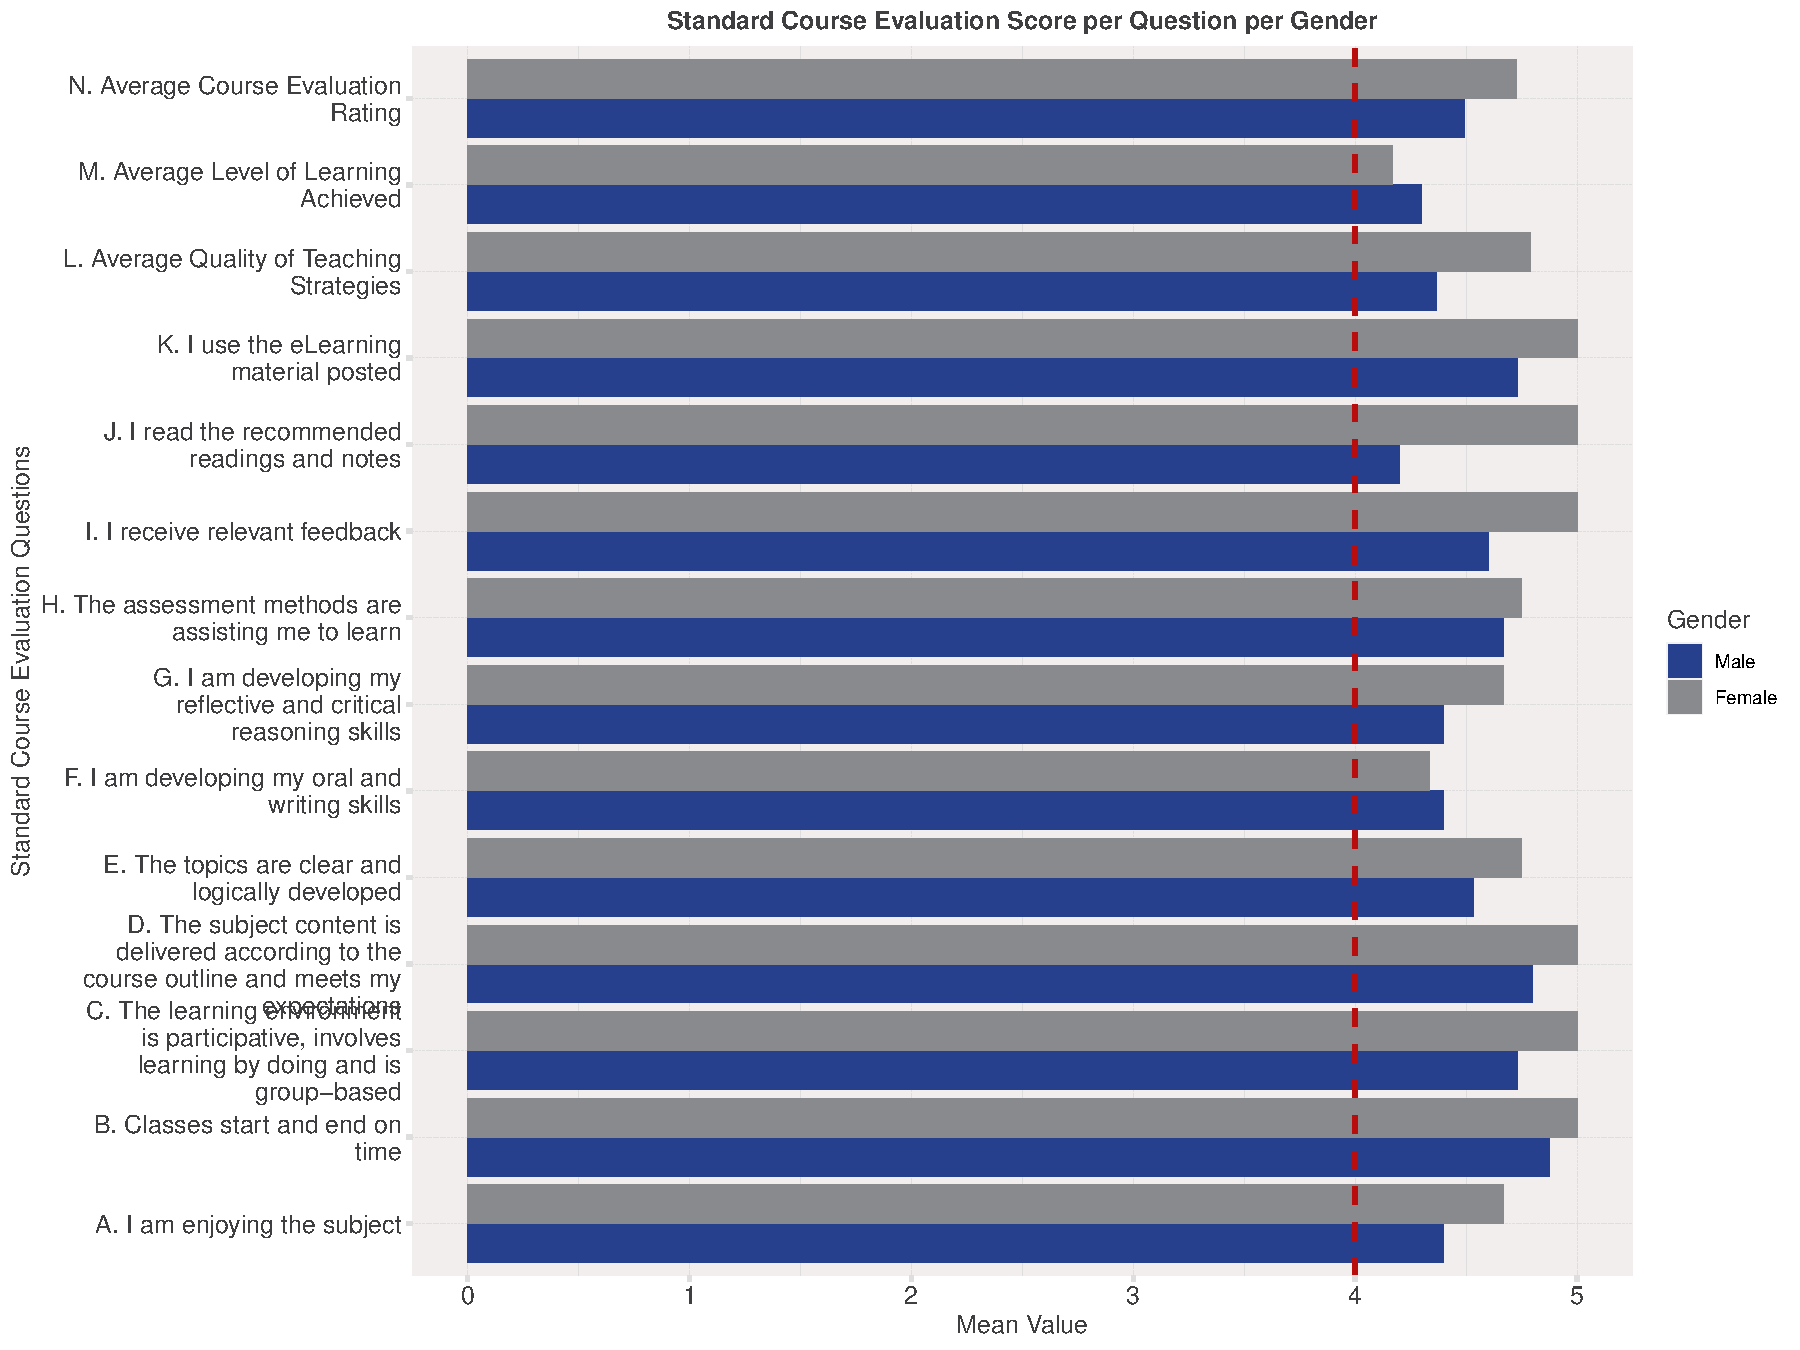
\includegraphics{AnalysisOfCourseEvaluation-Notebook_files/figure-latex/VisualizationsForCourseEvaluationResultsperGender-1.pdf}

\newpage

The plot below presents a drill-down of the class group into
\textbf{regular and exempt} students:

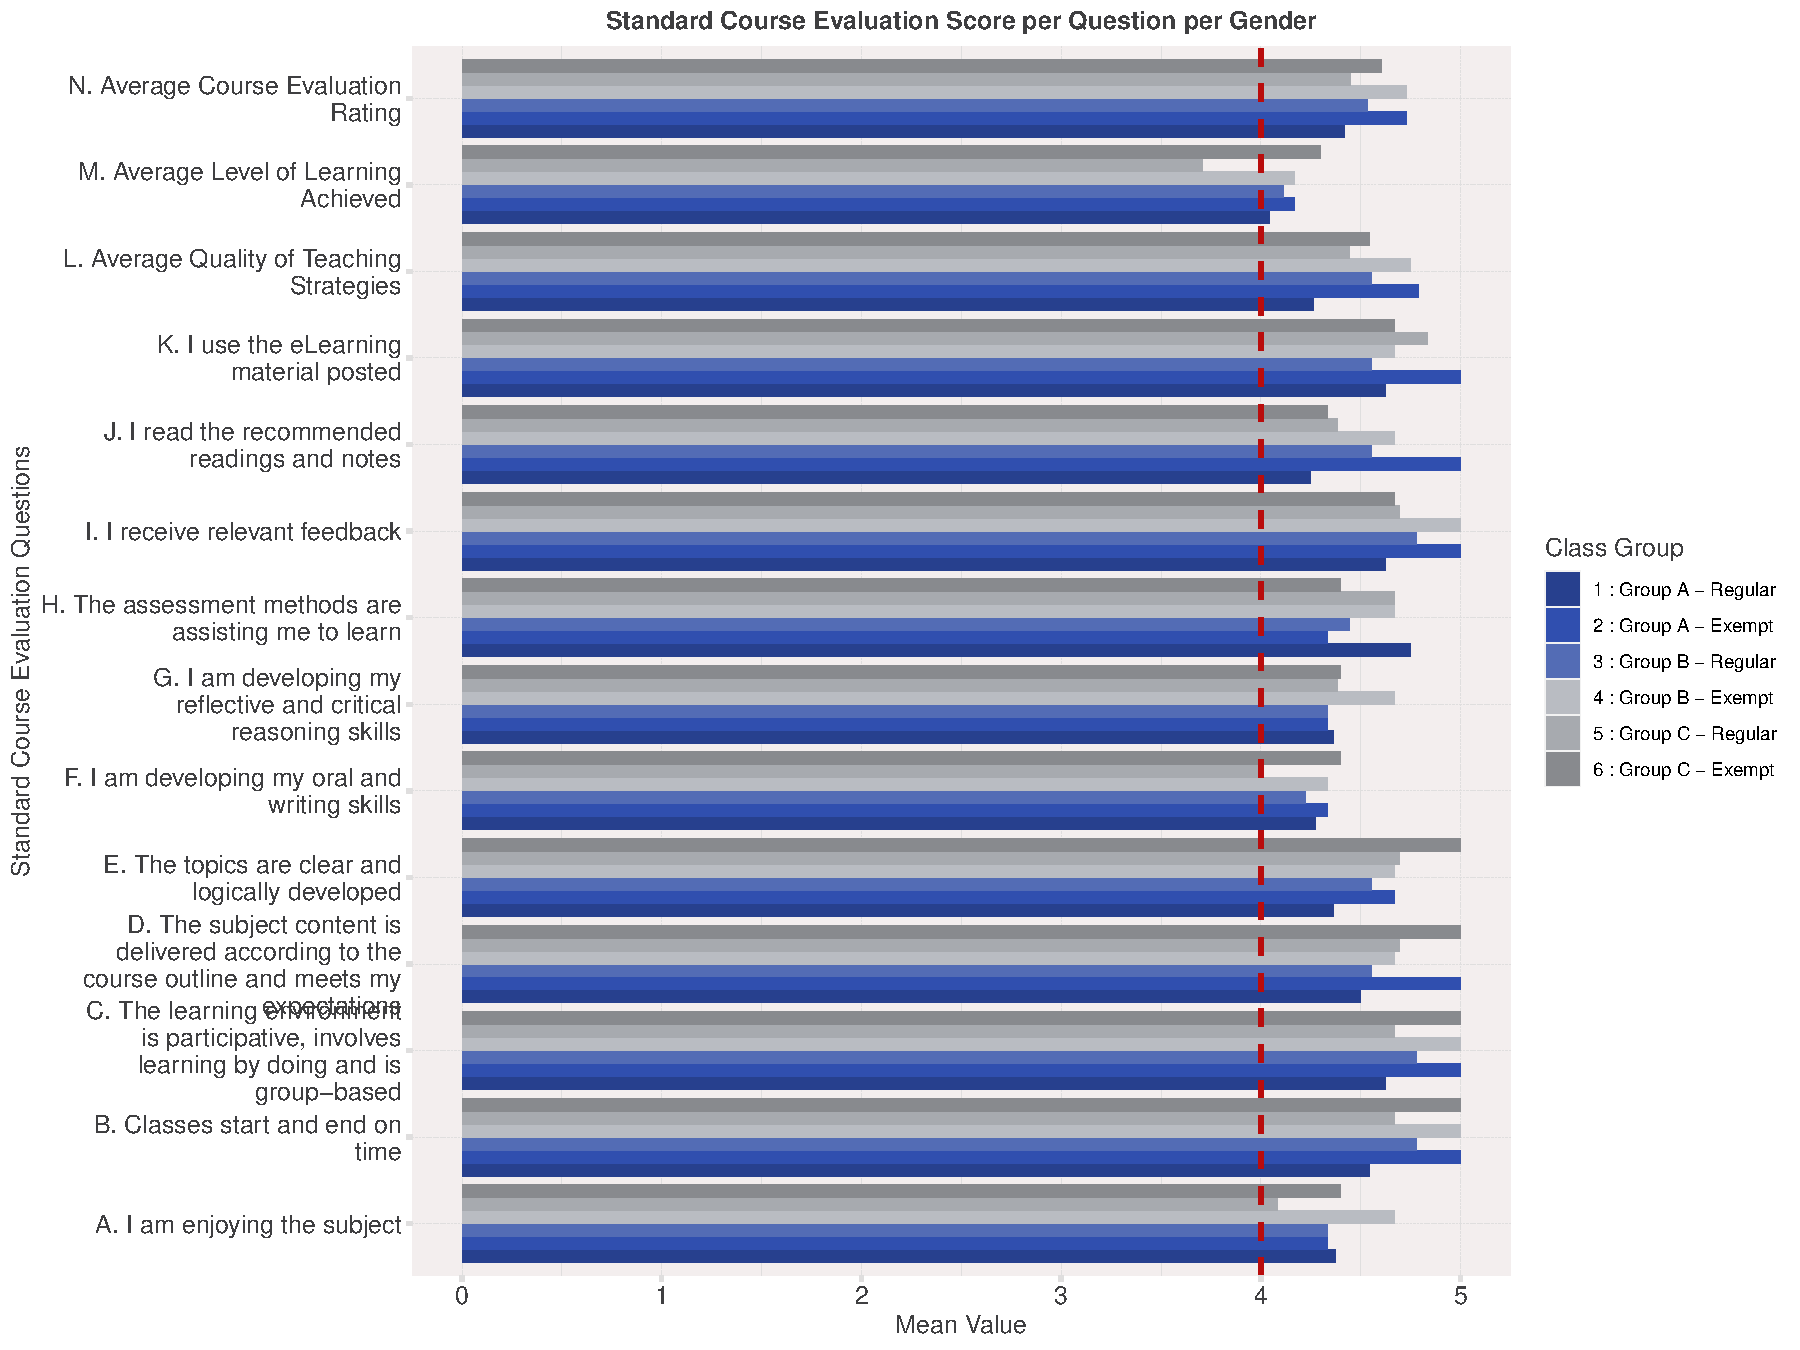
\includegraphics{AnalysisOfCourseEvaluation-Notebook_files/figure-latex/VisualizationsForCourseEvaluationResultsperGroup-1.pdf}

\newpage

\subsection{Correlations}\label{correlations}

The specific correlation values are presented below:

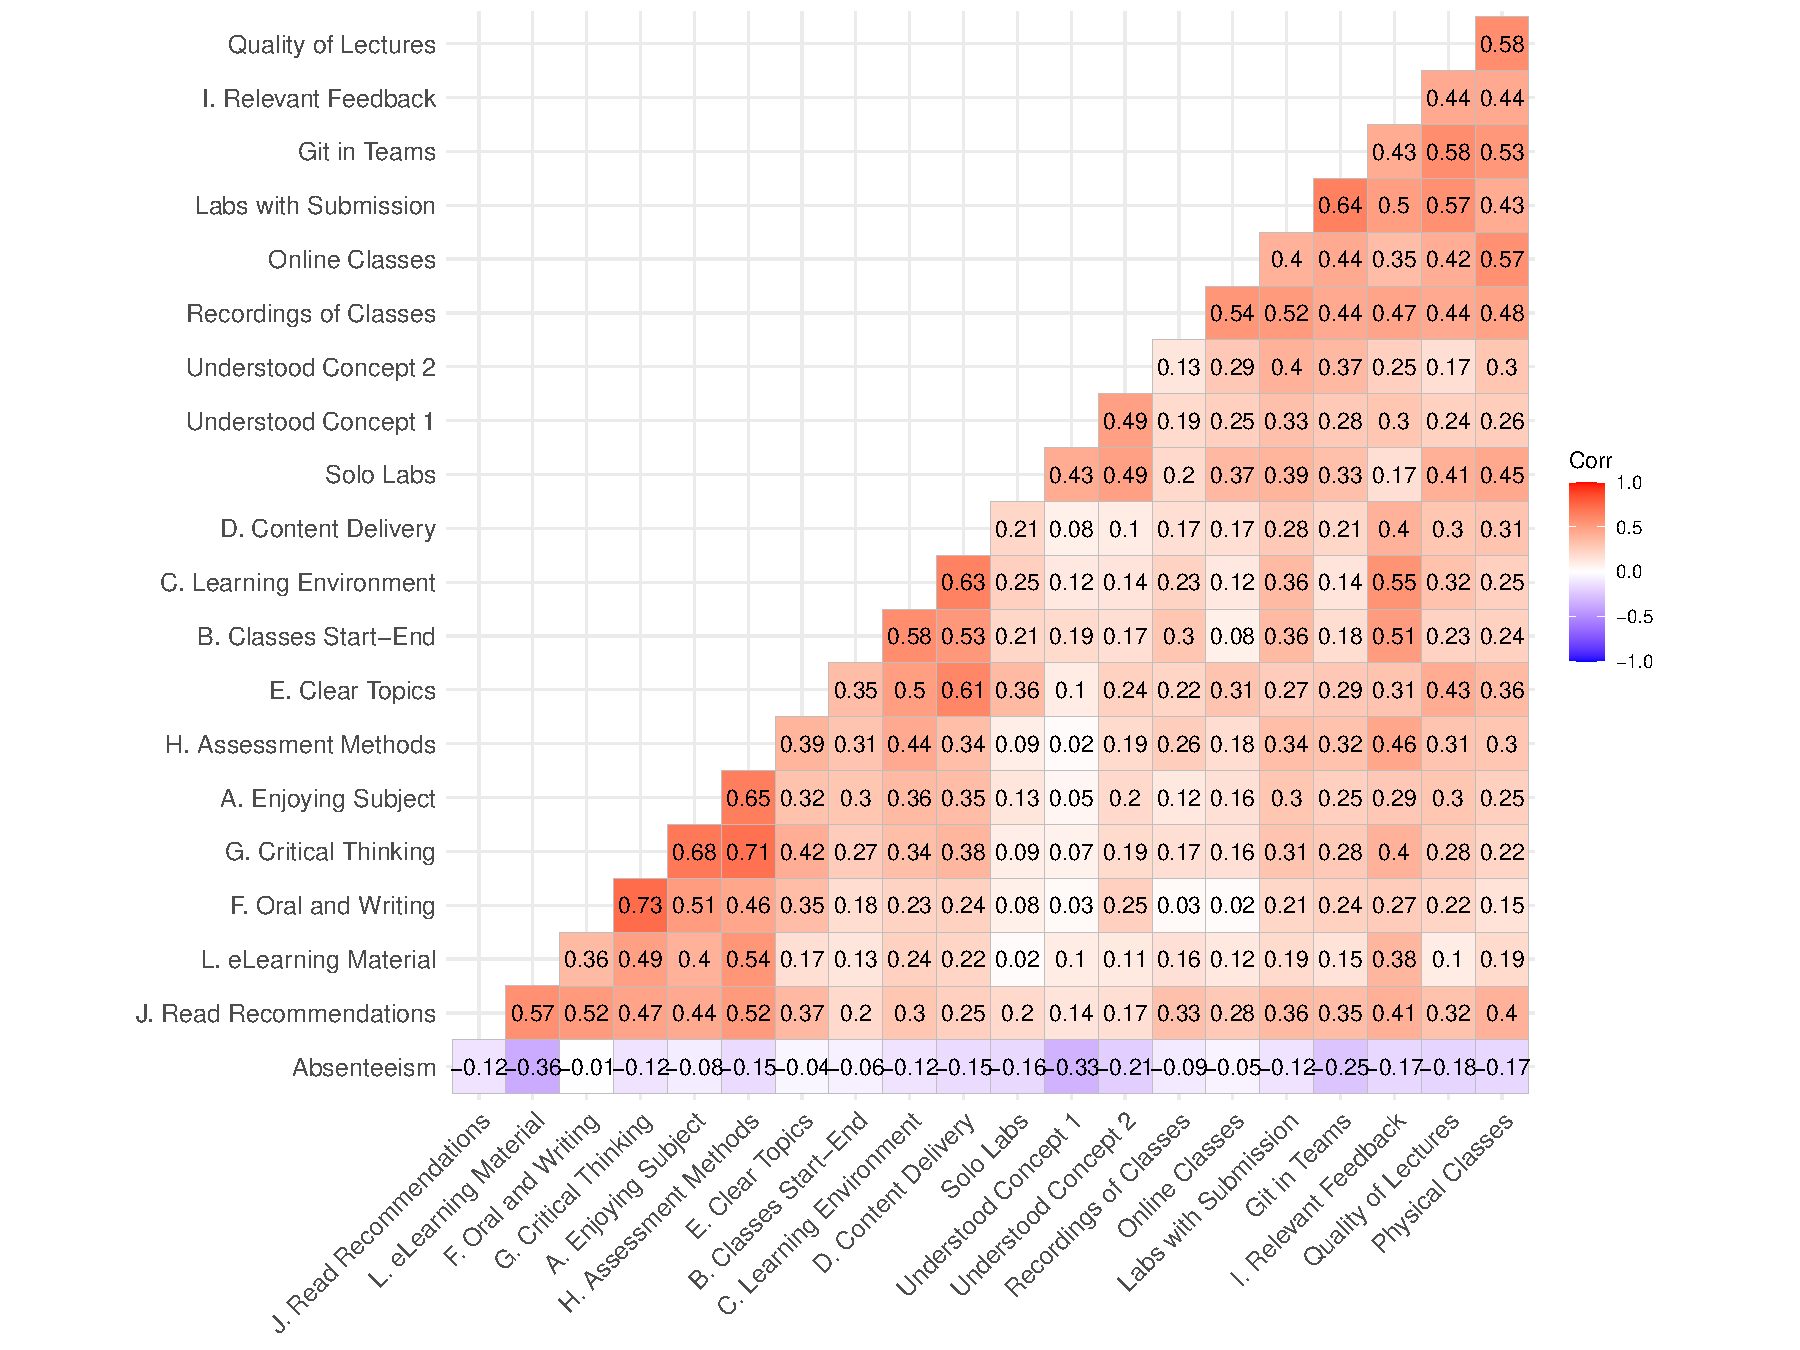
\includegraphics{AnalysisOfCourseEvaluation-Notebook_files/figure-latex/CorrelationMatrixWithFigures-1.pdf}

\subsubsection{Interesting Correlations}\label{interesting-correlations}

The following are hypothetical statements given that ``correlation does
not imply causation''.

\begin{itemize}
\item
  \textbf{.73 correlation} between ``I am developing my oral and writing
  skills'' and ``I am developing my reflective and critical reasoning
  skills'': \emph{Consider writing as formalized thinking.}
\item
  \textbf{.71 correlation} between ``The assessment methods are
  assisting me to learn'' and ``I am developing my reflective and
  critical reasoning skills'': \emph{The more effort students put into
  the assessment, the more they develop their reflective and critical
  reasoning skills.}
\item
  \textbf{.67 correlation} between ``I am enjoying the subject'' and ``I
  am developing my reflective and critical reasoning skills'': \emph{The
  more a student enjoys the subject, the more they consider their
  reflective and critical reasoning skills as developing.}
\item
  \textbf{.65 correlation} between ``The assessment methods are
  assisting me to learn'' and ``I am enjoying the subject'': \emph{The
  more interesting/challenging the assessment methods, the more students
  enjoy the course.}
\item
  \textbf{.63 correlation} between ``Labs that require you to use Git to
  work in a team'' and ``Labs that require you to put in effort to make
  a submission related to the content of the lab'': \emph{The more
  students appreciate the use of Git for working in teams, the more they
  appreciate labs that require a submission to be made.}
\item
  \textbf{.62 correlation} between ``The subject content is delivered
  according to the course outline and meets my expectations'' and ``The
  topics are clear and logically developed'': \emph{The more the course
  outline is followed, the clearer and more logically developed the
  topics are.}
\item
  \textbf{-.32 correlation} between ``Concept 1 of 4 - Ensemble Methods
  for Predictive Analytics'' and ``Absenteeism'': \emph{Students who
  started the semester late (high absenteeism), had a harder time
  understanding concept 1 which was covered at the beginning of the
  semester.}
\item
  \textbf{-.36 correlation} between ``I use the e-learning material
  posted'' and ``absenteeism'': \emph{The higher the number of classes
  missed, the lower the student's engagement with content posted on
  e-learning}
\end{itemize}

\begin{enumerate}
\def\labelenumi{(\arabic{enumi})}
\tightlist
\item
  A \textbf{.73 correlation} between ``I am developing my oral and
  writing skills'' and ``I am developing my reflective and critical
  reasoning skills'':
\end{enumerate}

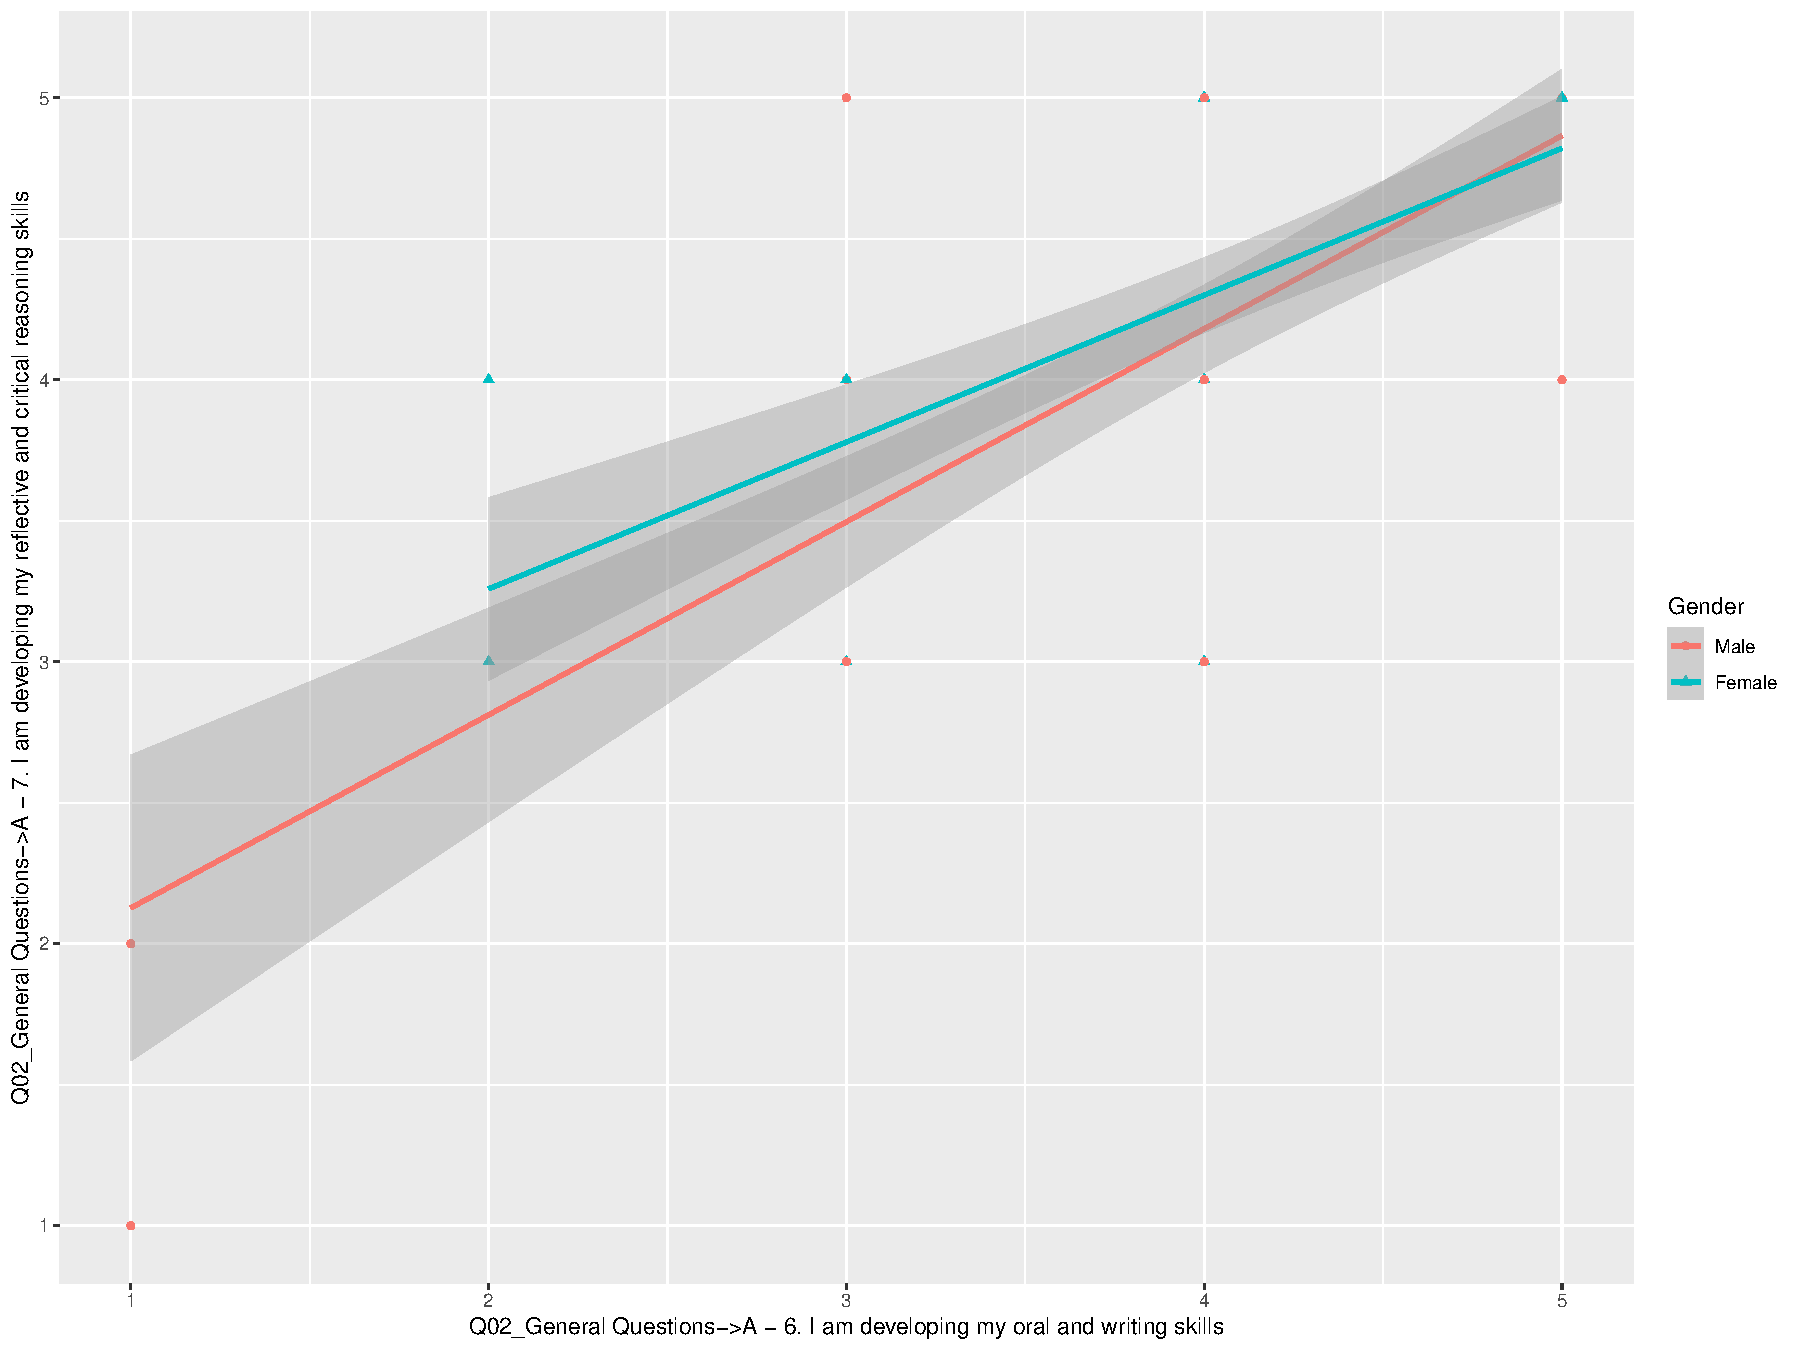
\includegraphics{AnalysisOfCourseEvaluation-Notebook_files/figure-latex/DrillDownCorr1-1.pdf}

\begin{enumerate}
\def\labelenumi{(\arabic{enumi})}
\setcounter{enumi}{1}
\tightlist
\item
  A \textbf{.71 correlation} between ``The assessment methods are
  assisting me to learn'' and ``I am developing my reflective and
  critical reasoning skills'':
\end{enumerate}

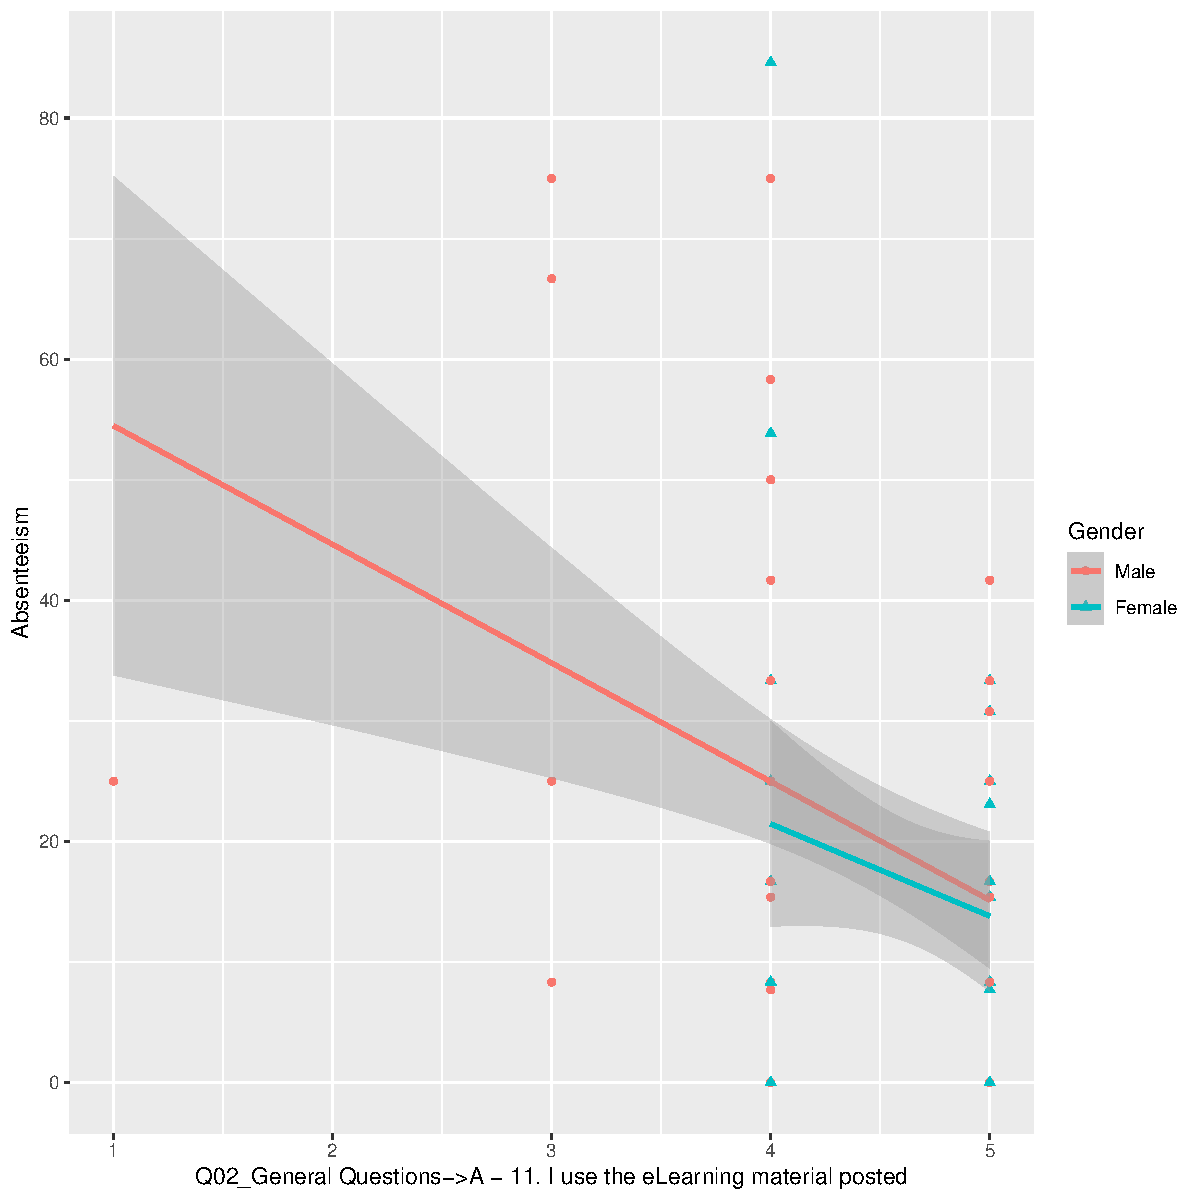
\includegraphics{AnalysisOfCourseEvaluation-Notebook_files/figure-latex/DrillDownCorr2-1.pdf}

\newpage

\subsubsection{Absenteeism Percentage}\label{absenteeism-percentage}

The lower the absenteeism, the more a student makes use of the
e-learning materials posted. And the more a student makes use of the
e-learning materials posted, the higher their overall grade in the
course.

With this in mind, a further investigation of the \textbf{absenteeism
percentage} is presented below.

\paragraph{Absenteeism by General Class
Group}\label{absenteeism-by-general-class-group}

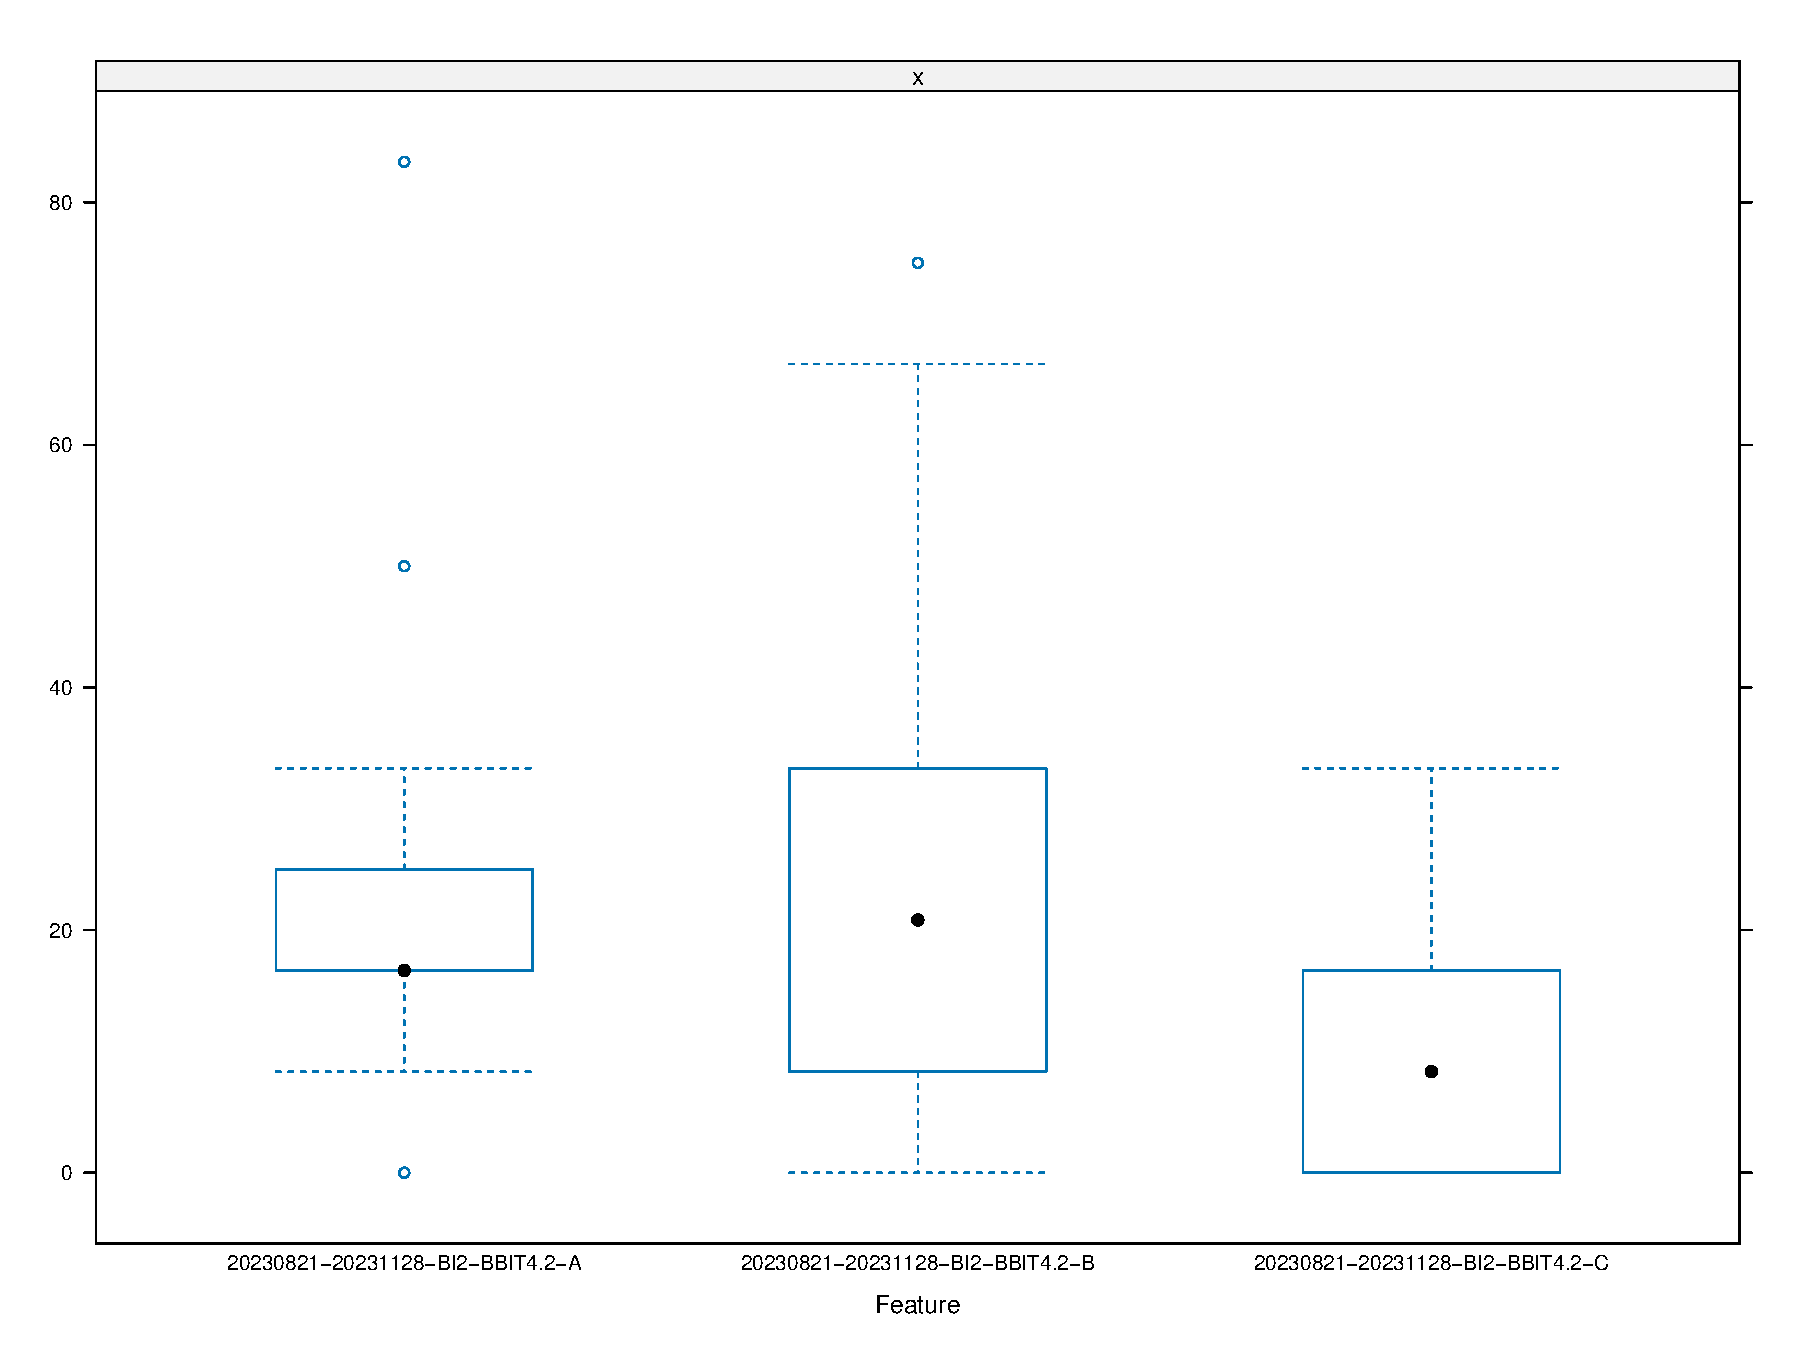
\includegraphics{AnalysisOfCourseEvaluation-Notebook_files/figure-latex/AbsenteeismBoxandWhiskerGroup-1.pdf}

\paragraph{Absenteeism by Specific Class
Group}\label{absenteeism-by-specific-class-group}

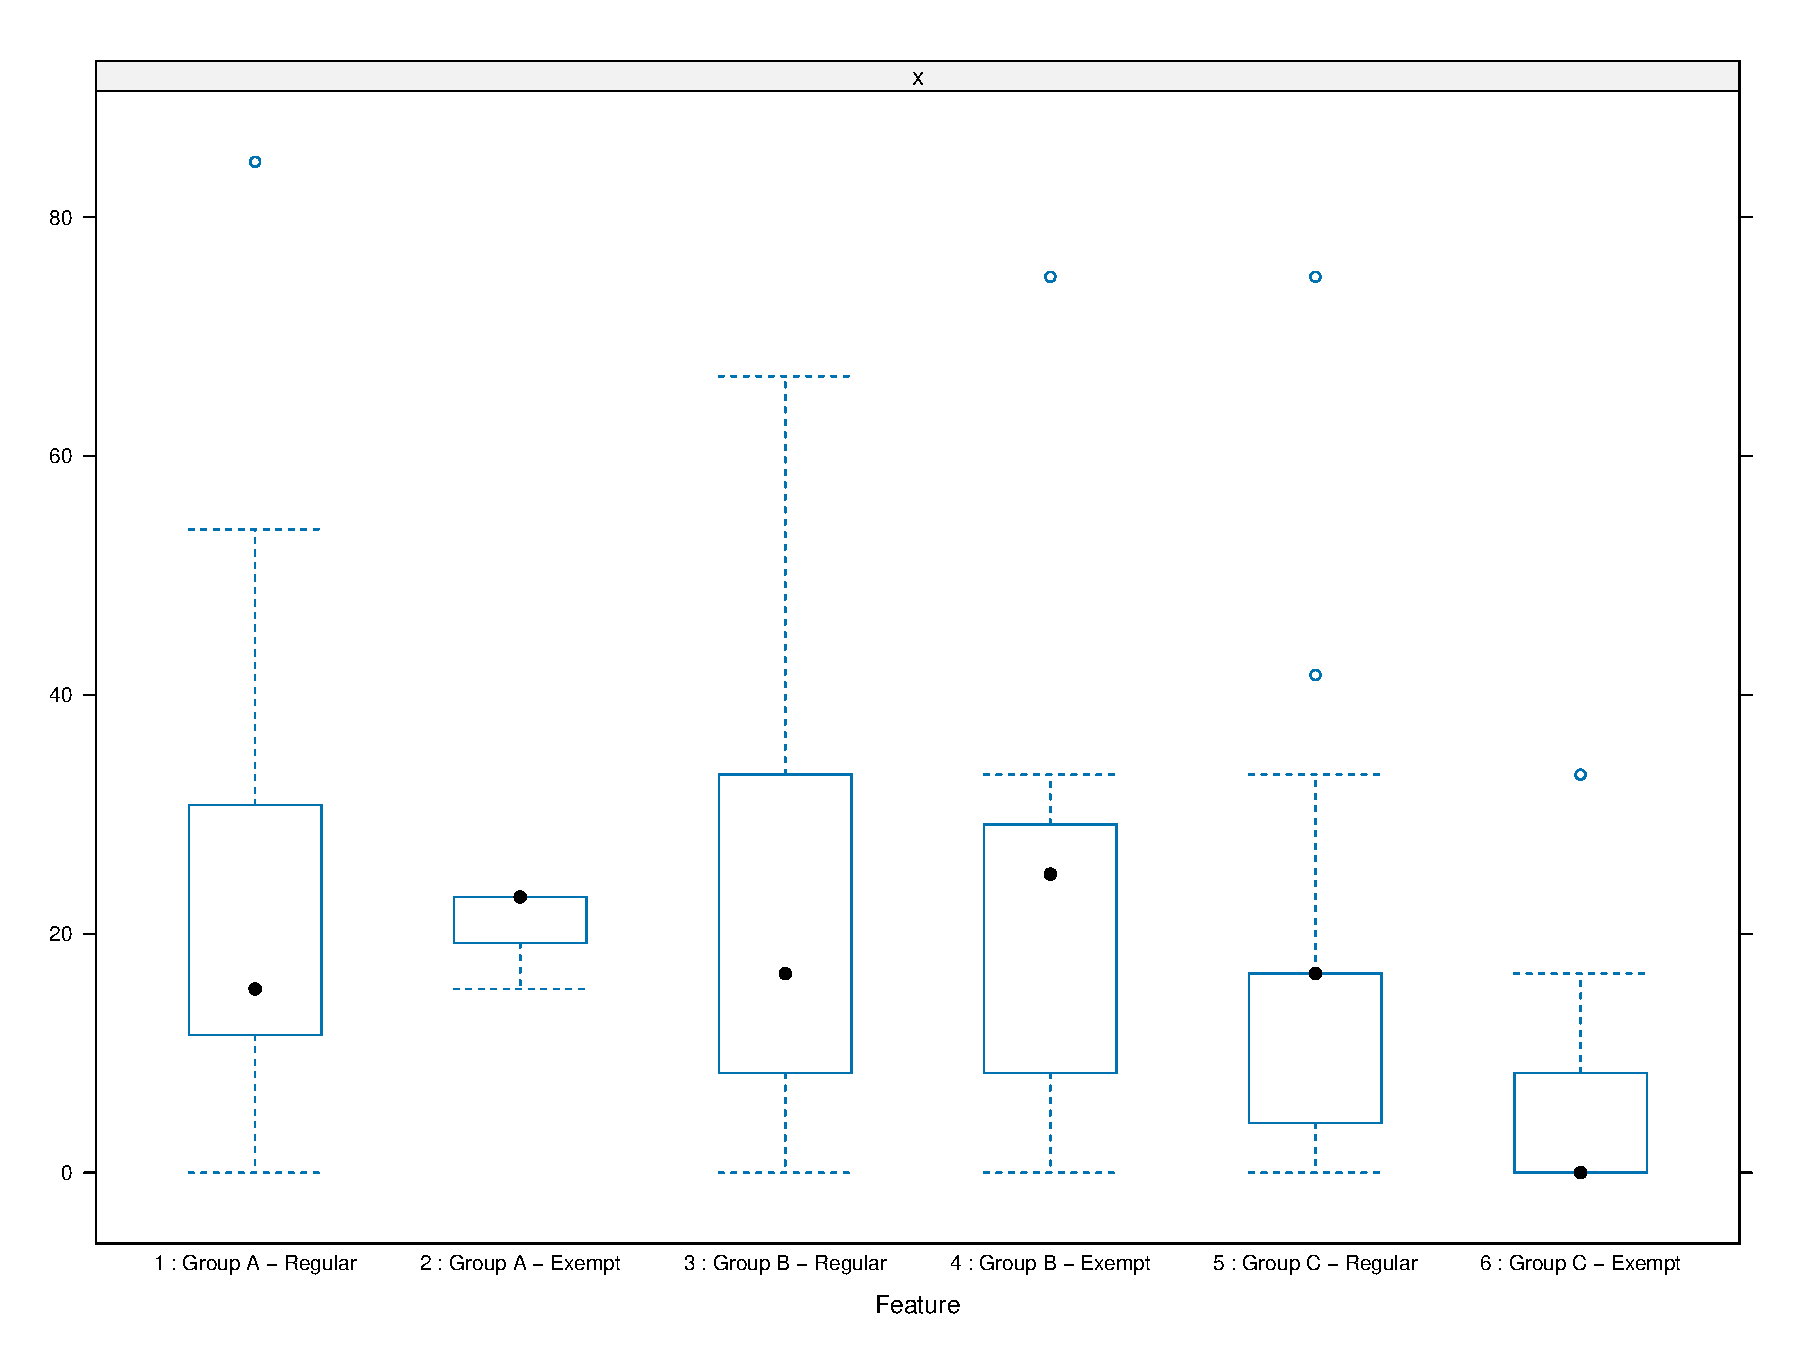
\includegraphics{AnalysisOfCourseEvaluation-Notebook_files/figure-latex/AbsenteeismBoxandWhiskerSpecificGroup-1.pdf}

\paragraph{Absenteeism by Gender}\label{absenteeism-by-gender}

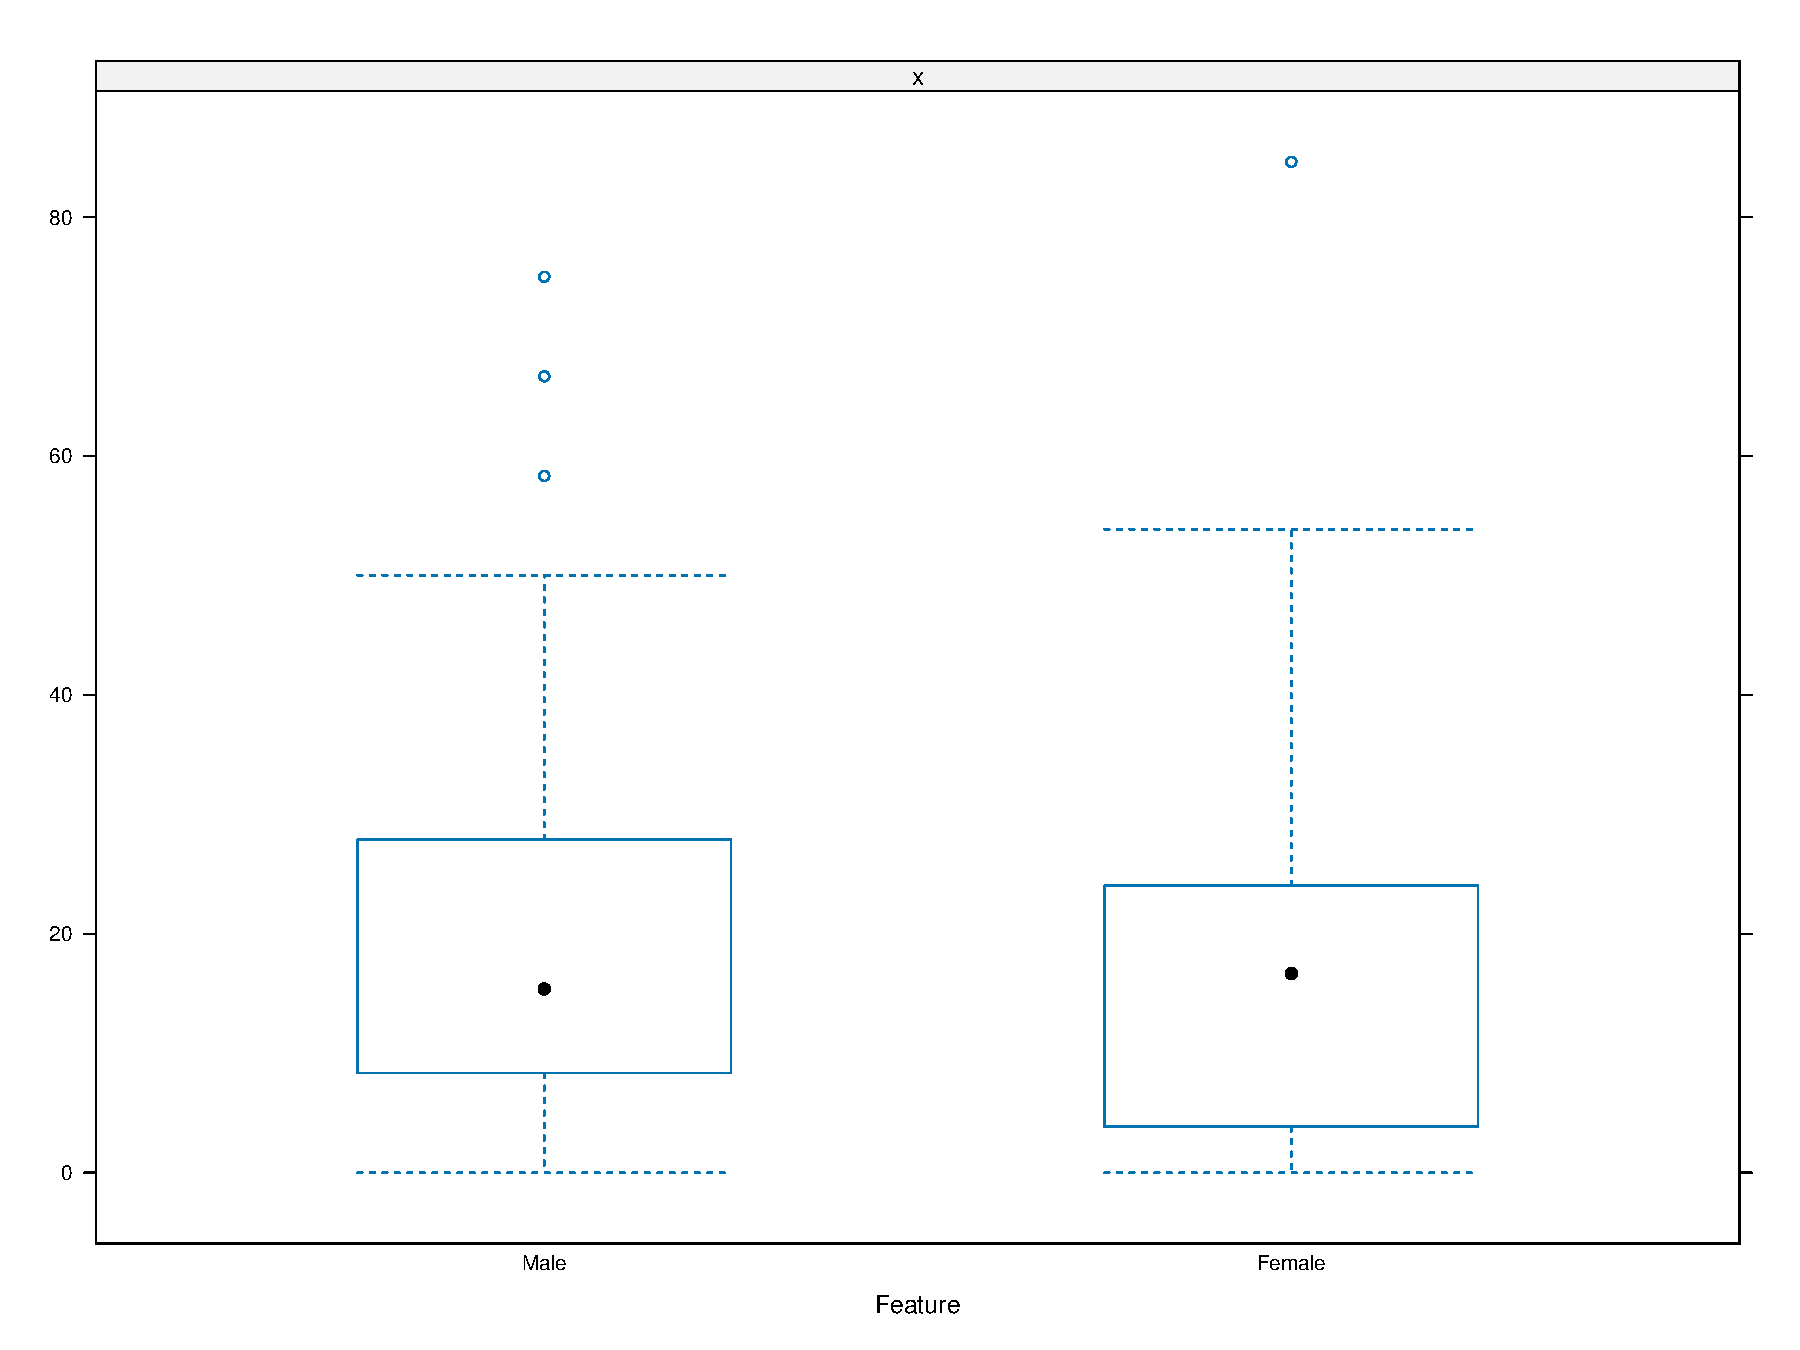
\includegraphics{AnalysisOfCourseEvaluation-Notebook_files/figure-latex/AbsenteeismBoxandWhiskerGender-1.pdf}

\newpage

\section{Qualitative Data Analysis}\label{qualitative-data-analysis}

\subsection{Sentiment Analysis
(Lexicon-Based)}\label{sentiment-analysis-lexicon-based}

The ``likes'' refer to the answer to the question, ``Write two things
you like about the teaching and learning in this unit so far.'' The
sentiments expressed through the ``likes'' are:

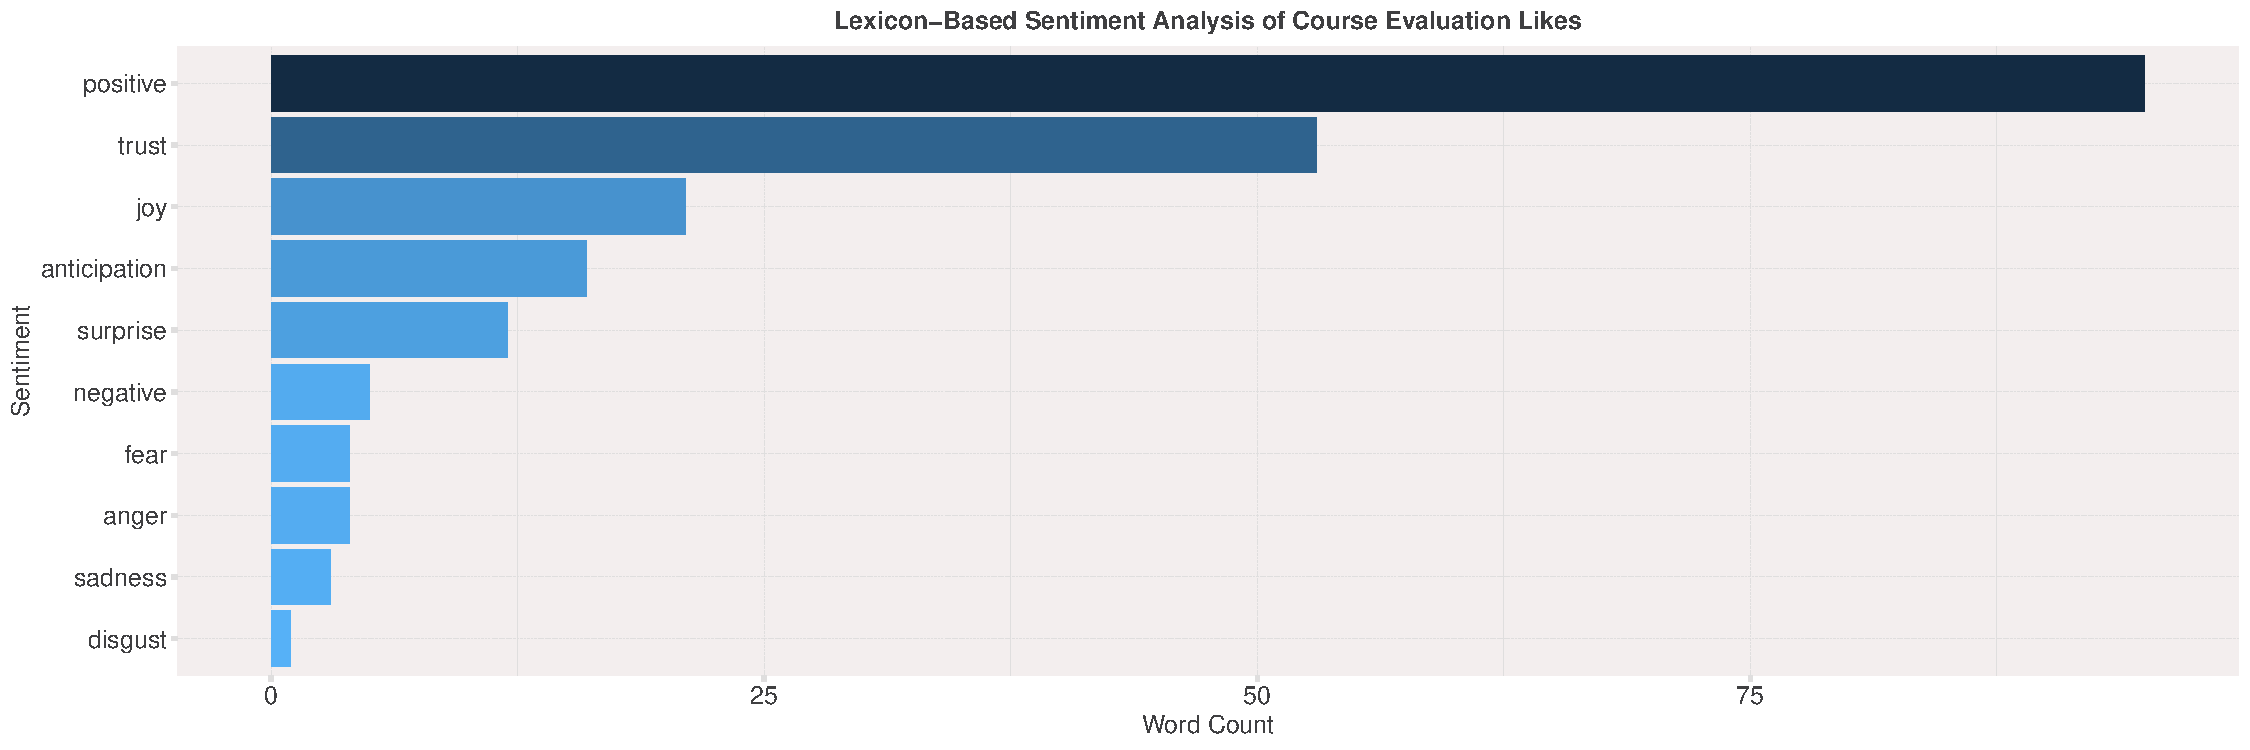
\includegraphics{AnalysisOfCourseEvaluation-Notebook_files/figure-latex/OverallSentimentForLikes-1.pdf}

The ``wishes'' refer to the answer to the question, ``Write at least one
recommendation to improve the teaching and learning in this unit (for
the remaining weeks in the semester).'' The sentiments expressed through
the ``wishes'' are:

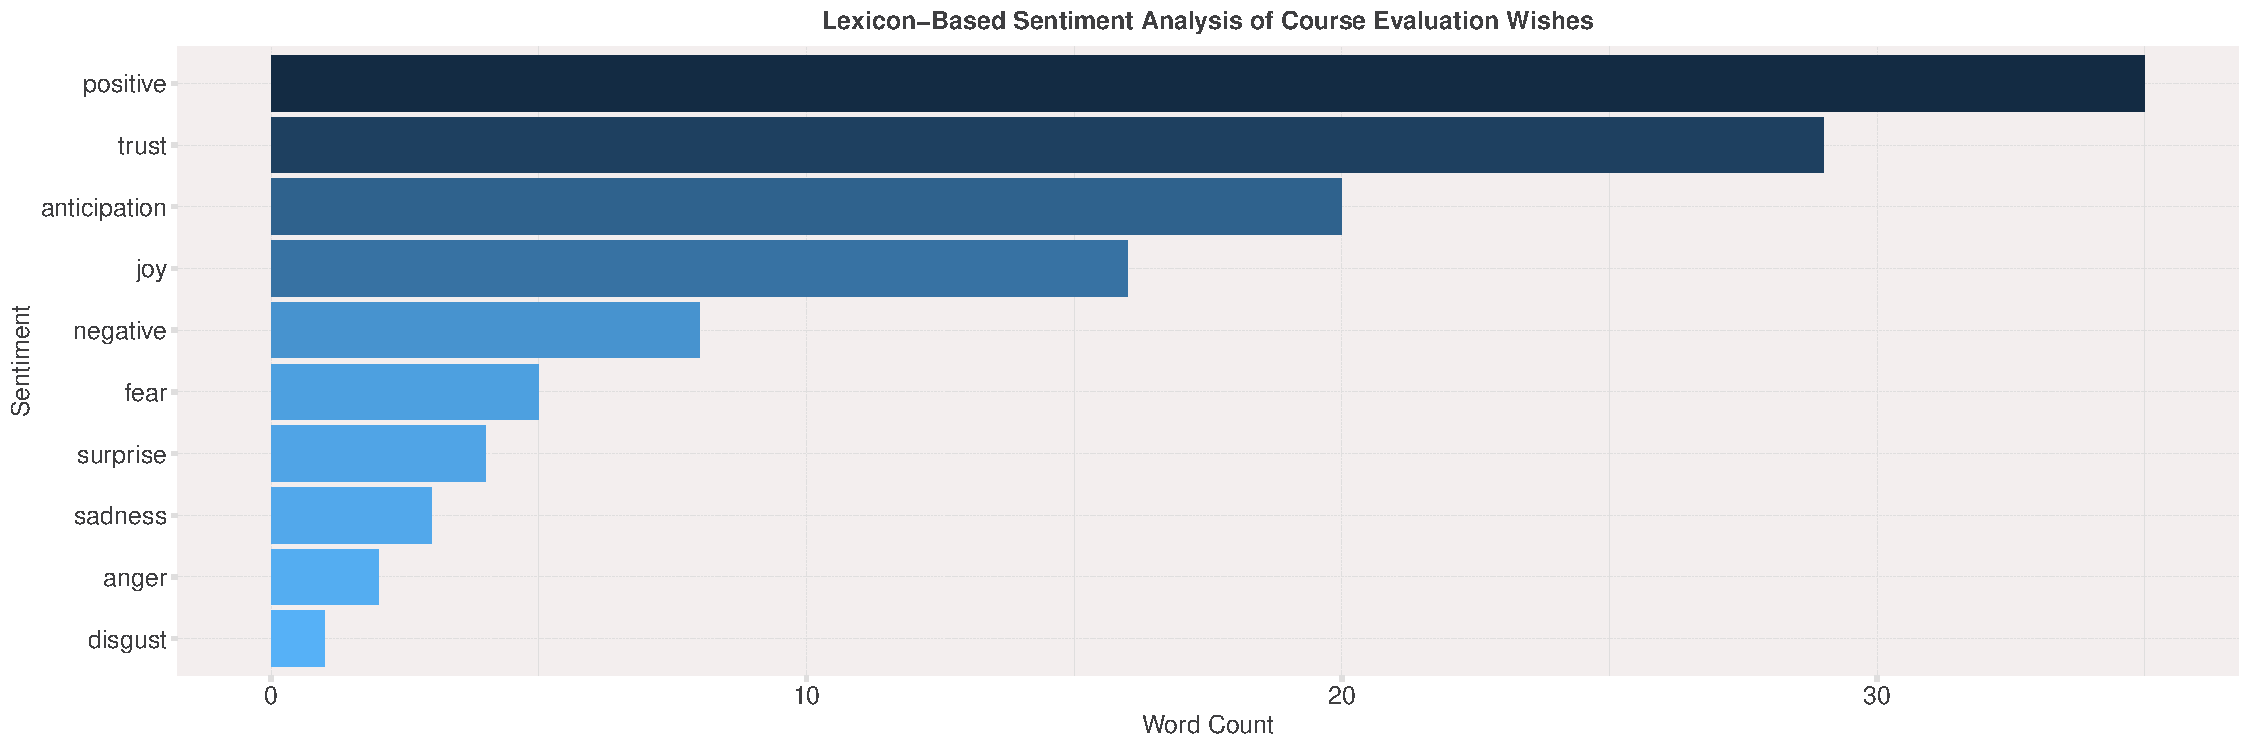
\includegraphics{AnalysisOfCourseEvaluation-Notebook_files/figure-latex/OverallSentimentForWishes-1.pdf}

\newpage

Chord Diagram of Likes per Class Group:

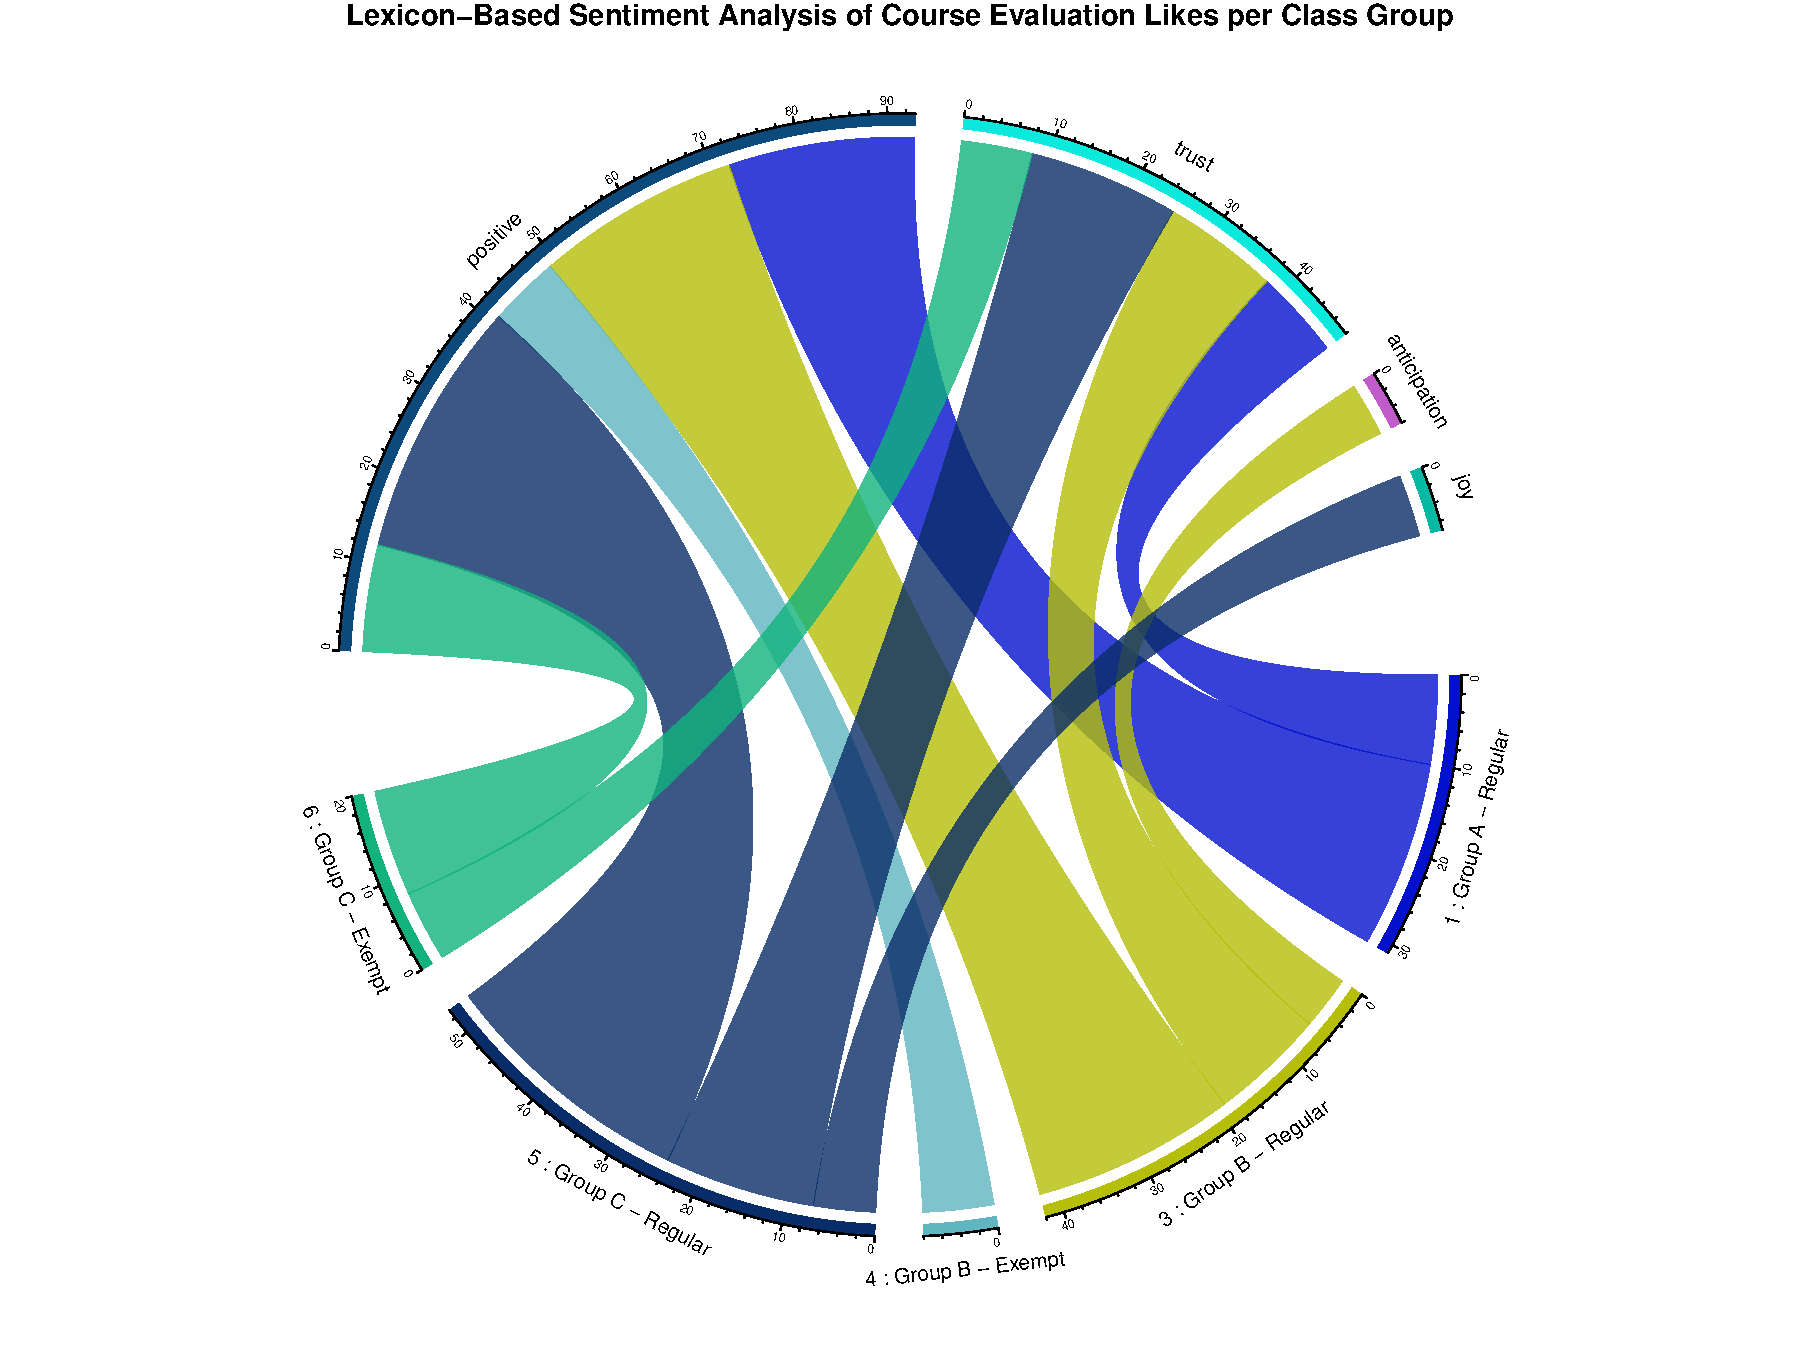
\includegraphics{AnalysisOfCourseEvaluation-Notebook_files/figure-latex/ChordDiagramLikesPerGroup-1.pdf}

\newpage

Chord Diagram of Likes per Class Gender:

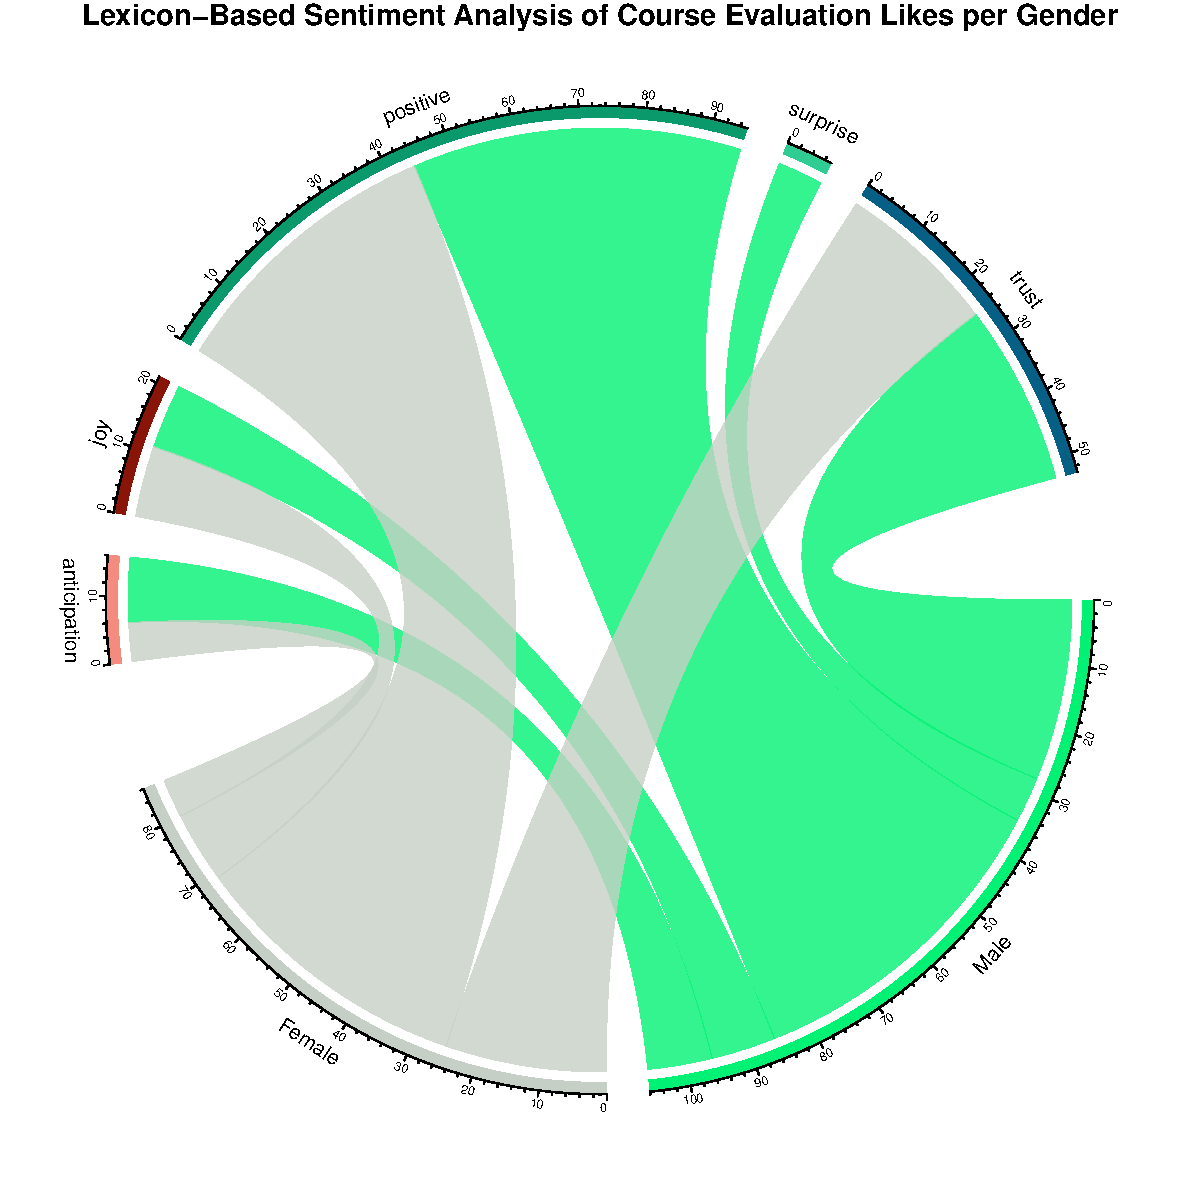
\includegraphics{AnalysisOfCourseEvaluation-Notebook_files/figure-latex/ChordDiagramLikesPerGender-1.pdf}

\newpage

Chord Diagram of Wishes per Class Group:

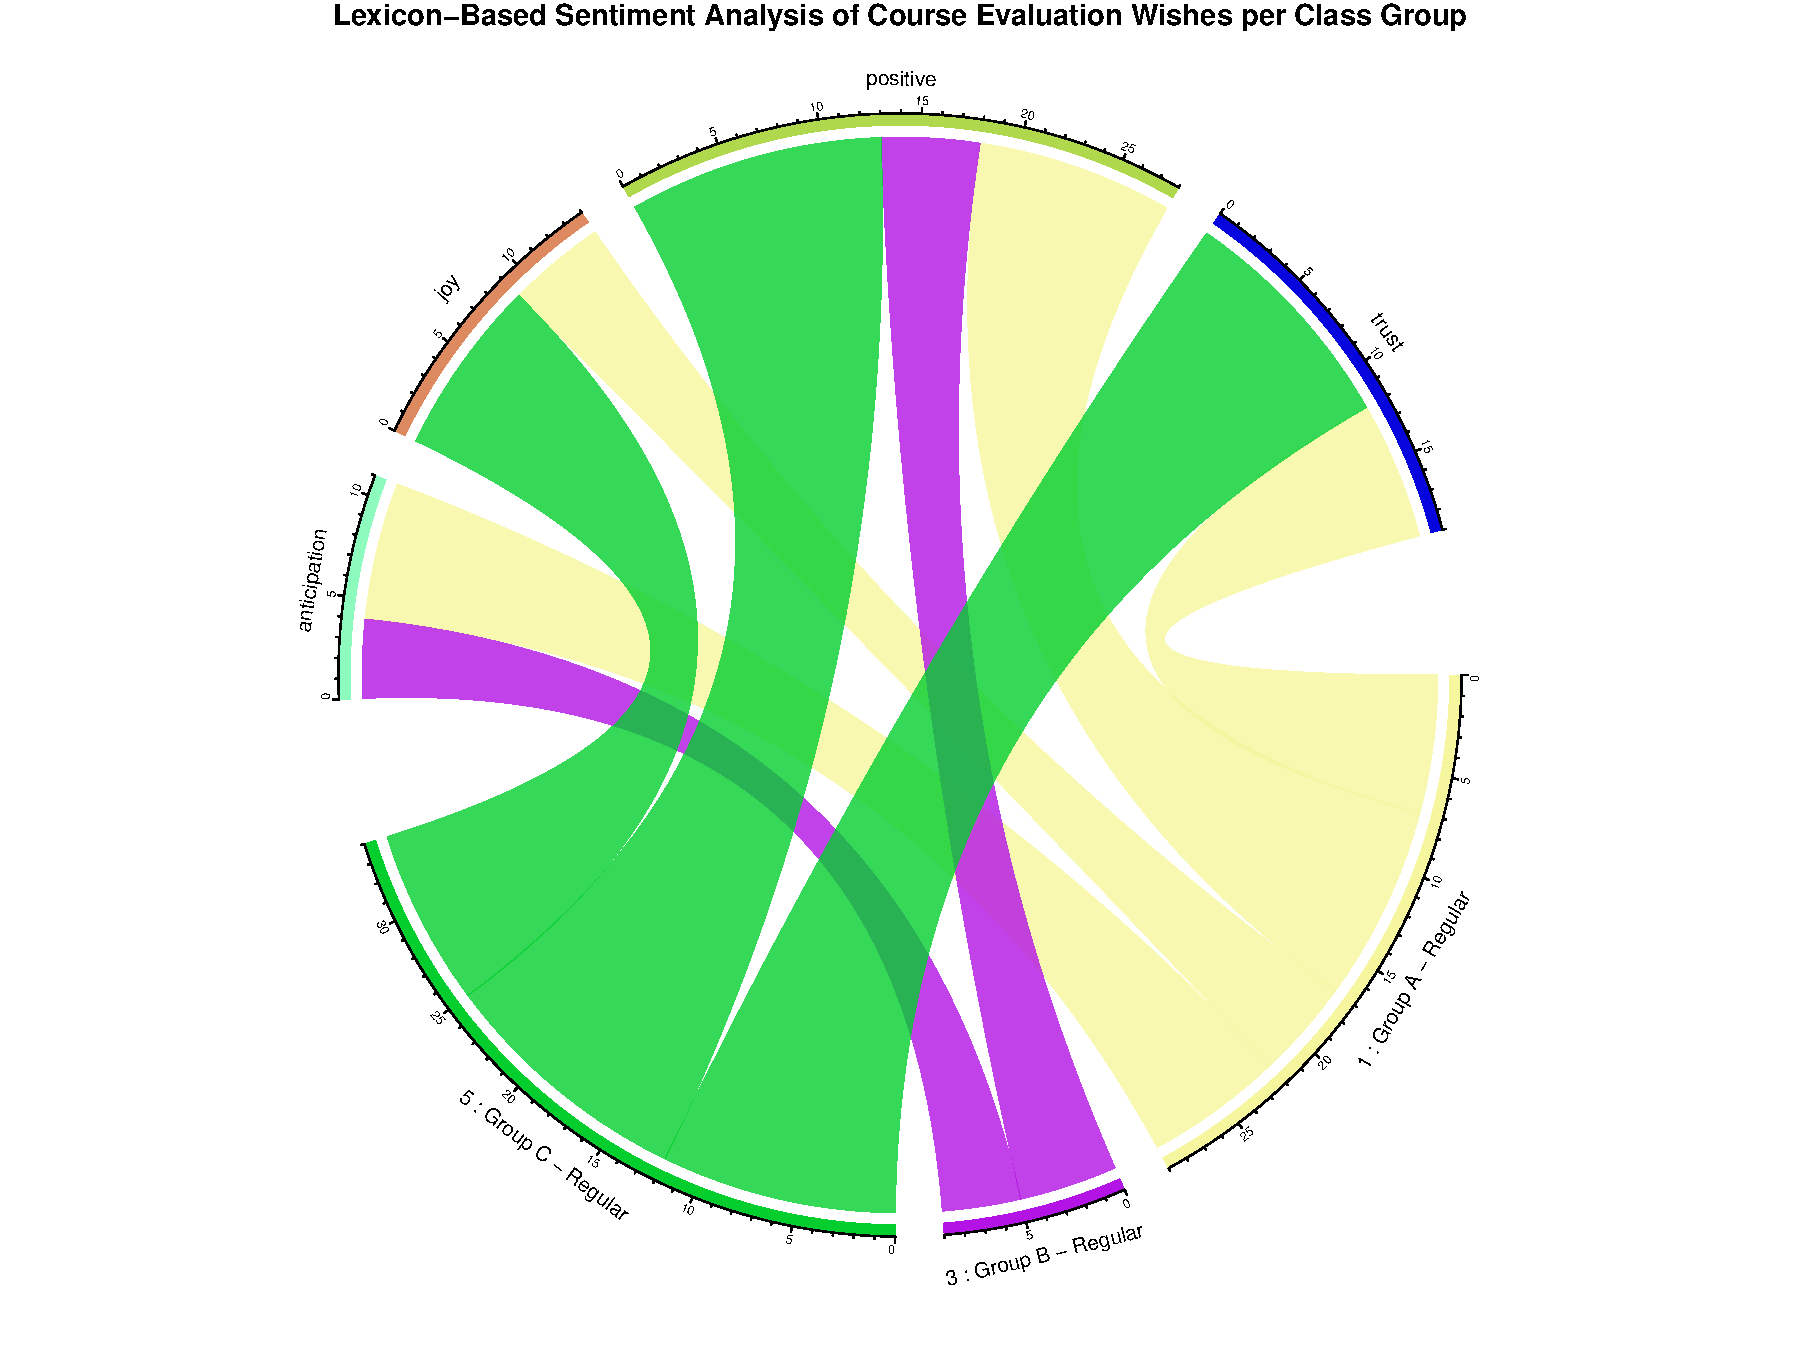
\includegraphics{AnalysisOfCourseEvaluation-Notebook_files/figure-latex/ChordDiagramPerGroup_Wishes-1.pdf}

\newpage

Chord Diagram of Wishes per Gender:

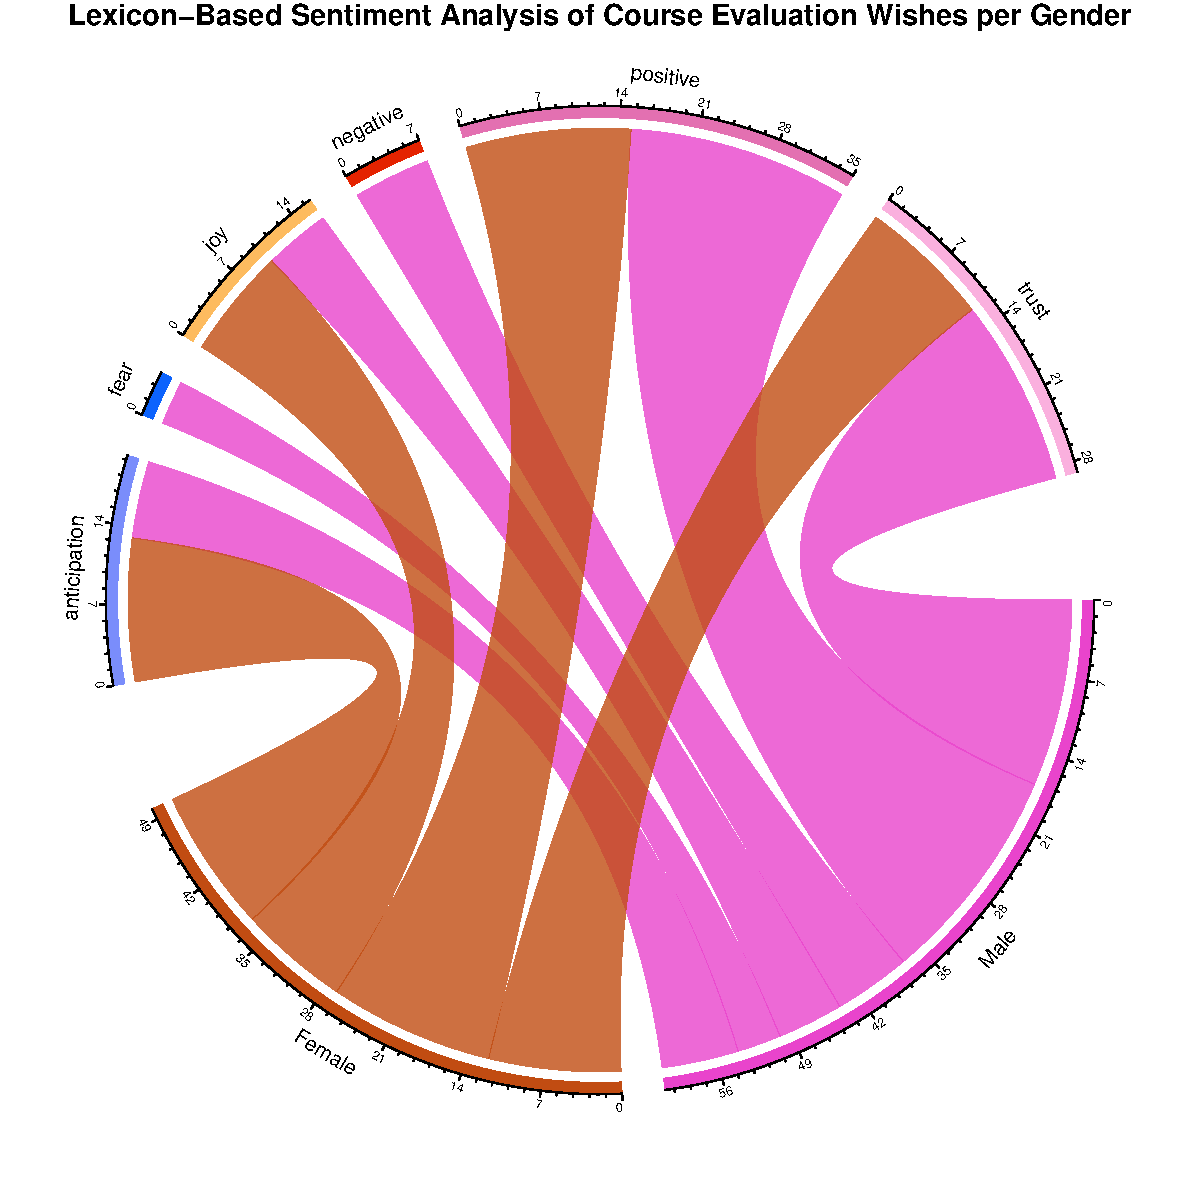
\includegraphics{AnalysisOfCourseEvaluation-Notebook_files/figure-latex/ChordDiagramPerGender_Wishes-1.pdf}

\newpage

\subsection{Topic Modelling (Latent Dirichlet Allocation (LDA)
based)}\label{topic-modelling-latent-dirichlet-allocation-lda-based}

The goal of topic modelling is to identify latent (hidden) terms
(topics) in the students' course evaluation textual feedback. In this
case, a topic is a mixture of words and a student's textual feedback is
a combination of one or more topics (mixed-membership model).

The 2 topics for the ``likes'' (as guided by the LDA model) are:

\begin{enumerate}
\def\labelenumi{\arabic{enumi}.}
\item
  Topic 1: Well-Explained Lectures
\item
  Topic 2: Interactive and Practical Labs
\item
  Topic 3: Learning Practical Skills
\end{enumerate}

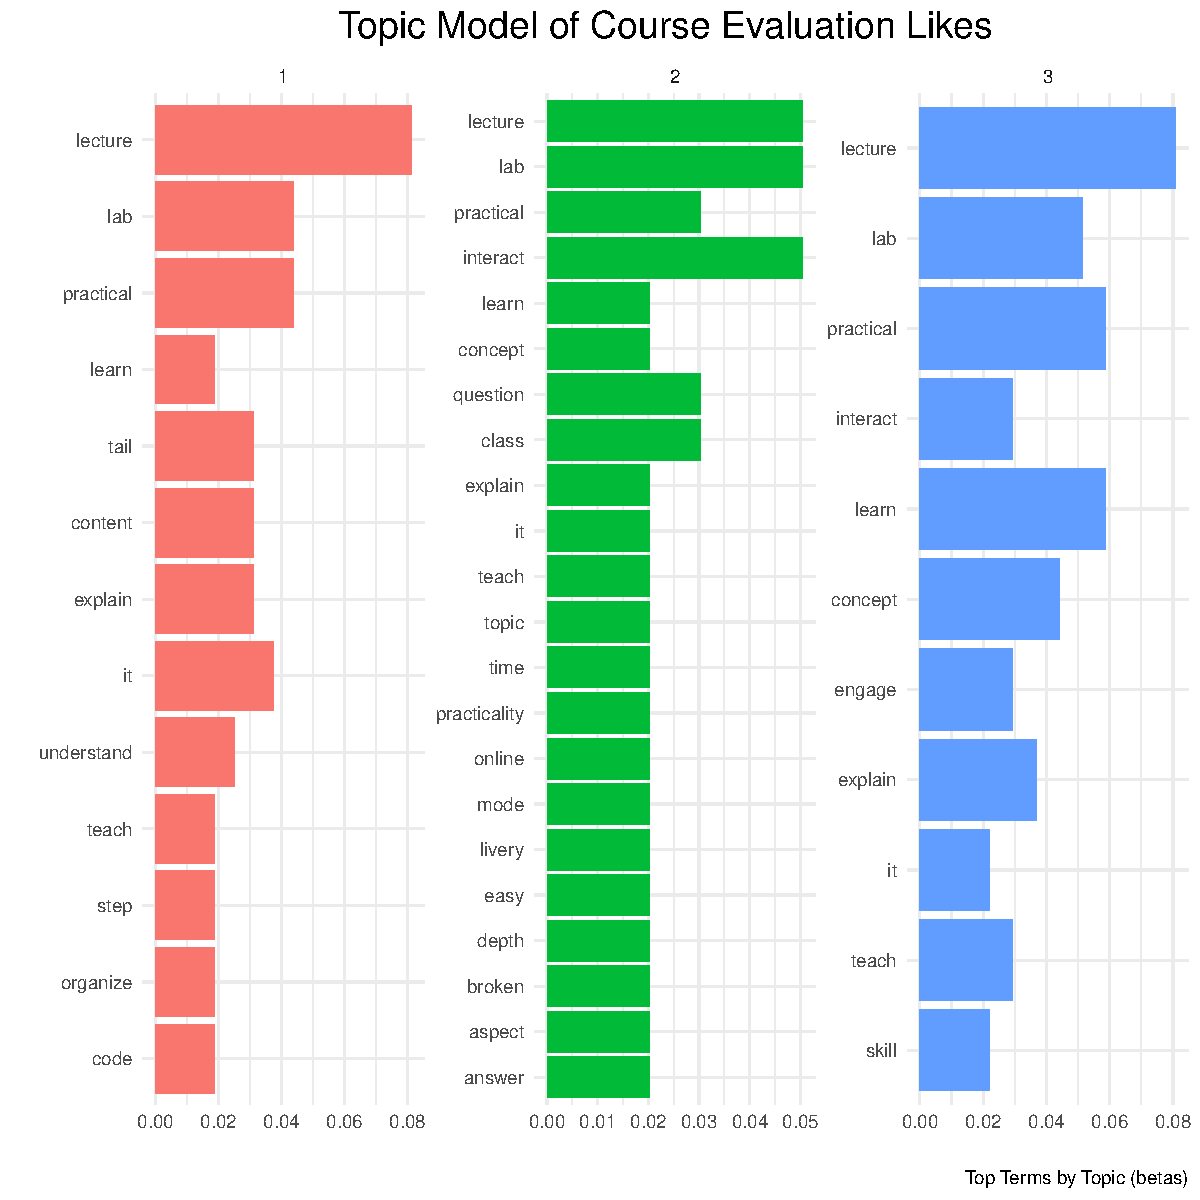
\includegraphics{AnalysisOfCourseEvaluation-Notebook_files/figure-latex/visualizations_for_likes_topic_modelling-1.pdf}

\newpage

The 5 topics for the ``wishes'' (as guided by the LDA model) are:

\begin{enumerate}
\def\labelenumi{\arabic{enumi}.}
\item
  Topic 1: Reduce the Amount of Content
\item
  Topic 2: Allocate More Time for the Labs
\item
  Topic 3: Lenient Deadlines
\item
  Topic 4: Recommend Professional Certifications
\item
  Topic 5: Help when Stuck in Technical Labs
\end{enumerate}

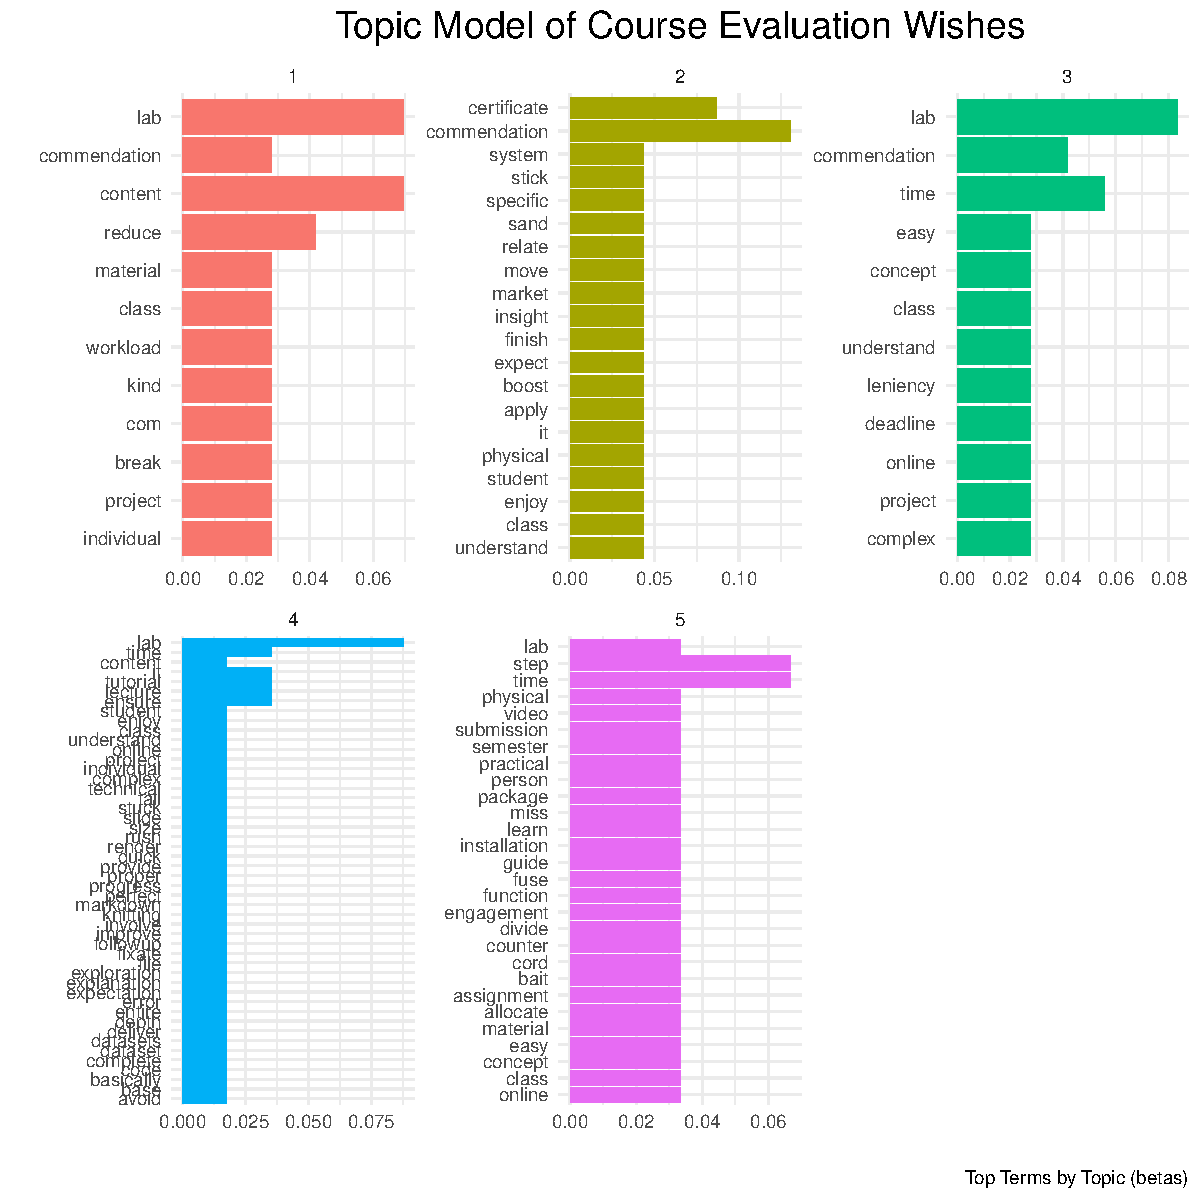
\includegraphics{AnalysisOfCourseEvaluation-Notebook_files/figure-latex/visualizations_for_wishes_topic_modelling-1.pdf}

\newpage

\section{Appendices}\label{appendices}

\subsection{Appendix A: Full Names of
Variables}\label{appendix-a-full-names-of-variables}

The following variables have been renamed to fit the correlation plots:

\begin{itemize}
\item
  `A. Enjoying Subject` = `Q02\_General Questions-\textgreater A - 1. I
  am enjoying the subject`,
\item
  `B. Classes Start-End` = `Q02\_General Questions-\textgreater A - 2.
  Classes start and end on time`,
\item
  `C. Learning Environment` = `Q02\_General Questions-\textgreater A -
  3. The learning environment is participative, involves learning by
  doing and is group-based`,
\item
  `D. Content Delivery` = `Q02\_General Questions-\textgreater A - 4.
  The subject content is delivered according to the course outline and
  meets my expectations`,
\item
  `E. Clear Topics` = `Q02\_General Questions-\textgreater A - 5. The
  topics are clear and logically developed`,
\item
  `F. Oral and Writing` = `Q02\_General Questions-\textgreater A - 6. I
  am developing my oral and writing skills`,
\item
  `G. Critical Thinking` = `Q02\_General Questions-\textgreater A - 7. I
  am developing my reflective and critical reasoning skills`,
\item
  `H. Assessment Methods` = `Q02\_General Questions-\textgreater A - 8.
  The assessment methods are assisting me to learn`,
\item
  `I. Relevant Feedback` = `Q02\_General Questions-\textgreater A - 9. I
  receive relevant feedback`,
\item
  `J. Read Recommendations` = `Q02\_General Questions-\textgreater A -
  10. I read the recommended readings and notes`,
\item
  `L. eLearning Material` = `Q02\_General Questions-\textgreater A - 11.
  I use the eLearning material posted`,
\item
  `Understood Concept 1` = `Q03\_Level of Learning
  Achieved-\textgreater B - 1. Concept 1 of 4 - Ensemble Methods for
  Predictive Analytics`,
\item
  `Understood Concept 2` = `Q03\_Level of Learning
  Achieved-\textgreater B - 2. Concept 2 of 4 - Predictive Modelling
  Using R`,
\item
  `Teaching - Labs` = `Q04\_Quality of Teaching
  Strategies-\textgreater C - 1. Labs with comments that describe each
  step to be followed`,
\item
  `Labs with Submission` = `Q04\_Quality of Teaching
  Strategies-\textgreater C - 2. Labs that require you to put in effort
  to make a submission related to the content of the lab`,
\item
  `Git in Teams` =`Q04\_Quality of Teaching Strategies-\textgreater C -
  3. Labs that require you to use Git to work in a team`,
\item
  `Solo Labs` = `Q04\_Quality of Teaching Strategies-\textgreater C - 4.
  Labs that require you to work alone`,
\item
  `Quality of Lectures` = `Q04\_Quality of Teaching
  Strategies-\textgreater C - 5. The quality of the lectures given
  (quality measured by the breadth (the full span of knowledge of a
  subject) and depth (the extent to which specific topics are focused
  upon, amplified, and explored) of learning - NOT quality measured by
  how fun/comical/lively the lectures are)`,
\item
  `Recordings of Classes` = `Q04\_Quality of Teaching
  Strategies-\textgreater C - 6. The recordings of online classes`,
\item
  `Online Classes` = `Q04\_Quality of Teaching Strategies-\textgreater C
  - 7. Online classes in general`,
\item
  `Physical Classes` = `Q04\_Quality of Teaching
  Strategies-\textgreater C - 8. Face-to-Face classes in general`
\end{itemize}

\subsection{Appendix B: Raw Qualitative
Data}\label{appendix-b-raw-qualitative-data}

\subsubsection{Likes}\label{likes}

The raw data of the likes is as follows:

\begin{longtable}[t]{>{\raggedright\arraybackslash}p{35em}}
\caption{\label{tab:RawLikesData}Write two things you like about the teaching and learning in this unit so far}\\
\toprule
Comment (Likes)\\
\midrule
It is interesting and helps improve coding skills\\
\hline
it is very detailed hence of great helpIt is interactive both in the unit and in regards to other units such as IS project II\\
\hline
 Ensemble Methods for Predictive Analytics   Predictive Modelling Using R \\
\hline
Interactive\\
\hline
The concepts are well explained  Communication is effective \\
\hline
It is a bit more practical due to the use of python and r  The instructor is well organized and the teaching methods are useful\\
\hline
It is practical and based on modern concepts  The labs are interesting and thought provoking\\
\hline
I like that the labs are practical  I like being given enough time to do the labs\\
\hline
Everything is good\\
\hline
It is interesting and interactive since we get to use different tools in our sessions.\\
\hline
So far its been a hard unit and fortunately the teaching style for the lecture is helping as he guides us along \\
\hline
Lecturer is efficient  classes start and end on time\\
\hline
Increase submission deadline \\
\hline
The practical labs are engaging hence skill development   the teaching method and lectures \\
\hline
1. It is comprehensive  2. It is interesting.\\
\hline
It is step by step   \\
\hline
- The content is really engaging and intense and shows that learning is there.  - Also additional hands on skills like using GitHub and collaborations which plays a huge role in the personal development goals in the digital space. \\
\hline
N/A\\
\hline
Interactivity and applicability of the unit\\
\hline
The online classes  The Labs that require submissions help me to dig deeper.\\
\hline
The practical examples and labs\\
\hline
The unit is very practical which helps me in the long run.  The lecturer does not leave anyone behind, ensures everyone has understood the concept\\
\hline
Work is clearly and easily broken down  The lecturer is very available for consultation\\
\hline
The teaching for this unit has been very comprehensive so far and engaging with the lecturer.  The learning implements group works.\\
\hline
Learning to use GIT  Being taught practically and through walk-throughs\\
\hline
The step by step explanation of the concepts is very helpful  The time to complete the labs is sufficient \\
\hline
The lec takes his time to teach the concept\\
\hline
Detailed Explanations.  Quick feedback by lecturer.\\
\hline
The labs are guided and help to learn  The lecturer is willing to repeat explaining areas of less understanding\\
\hline
The lecturer is readily available to help when one is stuck  The unit is well structured and organized\\
\hline
Very in depth  Very practical\\
\hline
Its practical and has interactive learning \\
\hline
It is interactive   It is engaging\\
\hline
The lecturer does everything in his power to ensure we are comfortable with content being taught and make sure we are following along together. The e-learning site is also very well organized and categorized for this unit\\
\hline
Answers the questions asked  Explains well\\
\hline
Patience and flow\\
\hline
mode of delivery  Information\\
\hline
The mode of delivery   The assistance of reference links put on elearning for easy reference \\
\hline
The lecturer ensures everyone understandsThe labs are fun\\
\hline
The lecturer ensures everyone has understood.  It is practical.\\
\hline
The explanations to the various concepts are well explained \\
\hline
the labs sessions are nice\\
\hline
i like the group labs  i like the topics\\
\hline
I find it current industry oriented\\
\hline
The lecturer provides adequate feedback on the questions asked.  The lab work clearly elaborates on the work taught.\\
\hline
The lecturer explains the content really well.\\
\hline
Takes time to organize his work, I appreciate the effort\\
\hline
So far so good  The lecturer is very clear\\
\hline
It is comprehensive  It is easy to follow\\
\hline
Labs that describe each step to be followed are engaging and learning enables me to follow through the lab properly  It is very engaging and interactive.\\
\hline
The lecturer asks questions  The lectures are clear \\
\hline
Interactive  Interesting \\
\hline
The content is very well delivered.\\
\hline
The assistance by the lecturer, the practicality\\
\hline
Lab work  Class sessions\\
\hline
 It is very participative and lecturer gives room for questions\\
\hline
feedback is quickLecturer is willing to help\\
\hline
Working as a team\\
\hline
the fact that we get to do the lab work in groups   the interactive online and on campus classes\\
\hline
I like how the Lecturer explains the concepts and takes us through the labs\\
\hline
The concept are explained very well  A chance to learn R I have wanting to interact with R and data\\
\hline
very interactive and hands on\\
\hline
on hand Practice  Good delivery\\
\hline
It’s interactive and very logical.\\
\hline
The technical aspect of the unit.  The attentiveness to detail when it comes to the labs and concepts are clearly explained.\\
\hline
i like the templates that come with the labs   i like the fact that we draw references from real world scenarios \\
\hline
Wide scope of content  Practicability\\
\hline
Once you follow the steps for the lab you will be okay.  The lecturer helps in one on one for the labs if one has an issue\\
\hline
The attention to detail when explaining the code. It makes it easier to understand  Having practical labs\\
\hline
I like the way the topics are broken down very logical and easy to understand.  I like that we are constantly able to ask questions and be answered regardless of the nature of the question.\\
\hline
The lectures\\
\hline
Its Good\\
\hline
the lecturer  the lectures\\
\hline
Lecturer, Teaching method\\
\hline
I like this ui=nit because it prompts me to think actually think and connect the dots \\
\hline
Well explained content\\
\hline
Gaining R skills\\
\hline
Use of realistic  code  group work\\
\hline
practicality  Engagement\\
\hline
Group Labs\\
\hline
its straight forward and simple to understand \\
\hline
I like the practicality of R and learning github in depth through the group work\\
\hline
Group workPractical Exercises\\
\hline
The learning of this unit is good in terms of the detailed and step by step practicals shown by the lecturer for each lab.The recordings.\\
\hline
The teaching is very thorough and labs have well explained instructions.\\
\hline
I like that it challenges me to apply everything practically.\\
\hline
None\\
\hline
The practical aspect.  The group work is good.\\
\hline
Labs activities, Quizzes help a lot on learning during the semester\\
\hline
clear and direct to the point   step by step teaching works for me\\
\hline
The lecturer explains everything in detail and caters for both ides that is vscode and rstudio\\
\hline
N/A\\
\hline
Systematic  Modular\\
\hline
N/A \\
\hline
How to use and implement R as a language for data analysis\\
\hline
I am learning to use new language, R language, and how to use it together with the available libraries for predictive analytics.   \\
\hline
Its practical \\
\hline
none\\
\hline
It is very practical and a good example of a prospective career path for many.\\
\hline
1. The lecturer makes the content easy to understand\\
\hline
the teaching method  the recording being online is also helpful \\
\hline
The practicals\\
\bottomrule
\end{longtable}

\newpage

\subsubsection{Wishes}\label{wishes}

The raw data of the wishes is as follows:

.begin\{longtable\}{[}t{]}\{\textgreater\{

\raggedright

\arraybackslash\}p\{35em\}\}
\textbackslash caption\{\label{tab:RawWishesData}Write at least one
recommendation to improve the teaching and learning in this unit (for
the remaining weeks in the semester).\textbackslash{} \toprule Comment
(Wishes)\textbackslash{} \midrule none\textbackslash{} \hline i would
like if the concepts were divided where we learn the functions first
online then do the practicals of it in person\textbackslash{} \hline
N/A\textbackslash{} \hline Flexibility\textbackslash{} \hline I don't
have any~\textbackslash{} \hline Leniency with regards to lab work
submission and future project work\textbackslash{} \hline More tutorials
based on the labs\textbackslash{} \hline Use of less complex
datasets\textbackslash{} \hline i have no
recommendations\textbackslash{} \hline A guide to help us counter
different problems like installation of packages during
labs.\textbackslash{} \hline I would like lab exercises to be done more
in class so as to easily understand~\textbackslash{} \hline Lecturer
might be a bit fast at times\textbackslash{} \hline Step by step
materials/videos on how to do the lab works~\textbackslash{} \hline
student involvement~~\textbackslash{} \hline
1. Nothing\textbackslash{} \hline Go easy on us abit, it is te last
semester\textbackslash{} \hline - To give us insights or recommendations
about certifications that we can as well do, related to this unit which
will boost our C.Vs for the interested students.~\textbackslash{} \hline
N/A\textbackslash{} \hline A bit more tutorials on technical errors such
as ones on knitting and rendering the markdown files\textbackslash{}
\hline If the concept requires many practicals, the classes should be
more online.\textbackslash{} \hline N/A\textbackslash{} \hline For the
physical class to be moved to a lab\textbackslash{} \hline Being more
lenient with lab work\textbackslash{} \hline Everything is okay so
far.\textbackslash{} \hline Sticking to a specific~application to be
used\textbackslash{} \hline No recommendation at the
moment\textbackslash{} \hline None\textbackslash{} \hline The content is
too broad and covers a lot i.e new softwares which make the unit
overwhelming.\textbackslash{} \hline More teamwork collaboration in
labs.\textbackslash{} \hline It would be better if the physical classes
were being recorded because at times one might be behind or missed an
important lab step ~\textbackslash{} \hline No
recommendations\textbackslash{} \hline N/A\textbackslash{} \hline Make
the course work less bulky and complex\textbackslash{} \hline no
comment\textbackslash{} \hline n/a.\\
\hline Too much content to deal with\textbackslash{} \hline time
liniency\textbackslash{} \hline That the labs should be given more time
to them~\textbackslash{} \hline Breaks in between
classes\textbackslash{} \hline Nothing. I am enjoying and understanding
the course.\textbackslash{} \hline None~\textbackslash{} \hline increase
more labs\textbackslash{} \hline the labs are quite hefty so it really
makes the work easier to do in a group\textbackslash{} \hline More
engagement\textbackslash{} \hline More time to be allocated in the lab
work assignments.\textbackslash{} \hline Nothing\textbackslash{} \hline
I am content\textbackslash{} \hline Reduce content Reduce
labwork\textbackslash{} \hline .\textbackslash{} \hline Proper detailed
explanation of the labs, rather than rushing through them quickly. More
time is needed for lab completion and progressive follow-up so the
lecturer knows where you are stuck.\textbackslash{} \hline More time for
labs\textbackslash{} \hline So far none\textbackslash{} \hline
-\textbackslash{} \hline Reduce the workload, its honestly too
much\textbackslash{} \hline More reference material Breaks during
classes at least 5 mins ~\textbackslash{} \hline None\ldots.The unit met
my expectation and was delivered perfectly\textbackslash{} \hline Avoid
online classes\textbackslash{} \hline Deadlines to be extended
abit\textbackslash{} \hline N/A\textbackslash{} \hline i am enjoying the
unit as it is\textbackslash{} \hline Since we are about to finish our
8.4.4 system. To give us more recommendation on certificates and what
the job market expects from us\textbackslash{} \hline better
communication of activities btwn the students and the
lec~\textbackslash{} \hline .\textbackslash{} \hline Ensure that the
code work can work with any dataset and not fixated on provided
dataset\textbackslash{} \hline I would like there be more simpler labs
with easier datasets to understands the concepts first then move on to
more complex data handling and manipulation.\textbackslash{} \hline i
wish that that the lab assignments could be allocated more time, that
they are marked towards the end of the semester~ ~\textbackslash{}
\hline None so far\textbackslash{} \hline Kindly share more reading
materials and past papers.\textbackslash{} \hline Having more practical
labs\textbackslash{} \hline I recommend that the deadlines on the labs
be more flexible as there are many subject and projects running
concurrently.\textbackslash{} \hline The labs are long, they are
individually basically the same size as an entire same
project\textbackslash{} \hline No recomendation\textbackslash{} \hline
so far so \vphantom{1} good\textbackslash{} \hline Greater in depth
exploration into labs to ensure we're actually understanding what is
going on.\textbackslash{} \hline The content is so hard to understand
and the lec solving other people's issues only bring more confusion to
some of us. I wish he would go through the content first then afterwards
focus on individual problems\textbackslash{} \hline He is doing a good
job\textbackslash{} \hline Personally I use linux and its kinda hard for
me~ You can add some YouTube materials~\textbackslash{} \hline Lab
submissions still very confusing\textbackslash{} \hline More online
sessions\textbackslash{} \hline None\textbackslash{} \hline so far so
good\textbackslash{} \hline Adequate time for completing the
labs\textbackslash{} \hline More group work, less individual
work\textbackslash{} \hline ~No recommendations there is good
delivery.\textbackslash{} \hline Generally just slow down the amount of
work we have to submit considering the IS project we need to work
on\textbackslash{} \hline One recommendation may be to explain how these
concepts can relate to and apply to our IS Project 2.\textbackslash{}
\hline None\textbackslash{} \hline It is okay.\textbackslash{} \hline -
Slide are very long (too much content) lecture can improve on
that-\textbackslash{} \hline nothing really\textbackslash{} \hline There
are many labs\textbackslash{} \hline N/A\textbackslash{} \hline Further
work on ease of following the lab work\textbackslash{} \hline
N/A\textbackslash{} \hline No comment, everything is
fine\textbackslash{} \hline None\textbackslash{} \hline nothing all is
well\textbackslash{} \hline reduce the workloads on the labs
kindly\textbackslash{} \hline n/a.\textbackslash{} \hline
N/A\textbackslash{} \hline so far I have been struggling a little with
the Lab a bit but i'm hoping it will get better as we continue with the
other labs\textbackslash{} \hline N/A\textbackslash{} \bottomrule
\textbackslash end\{longtable\}

\end{document}
